\documentclass{report}

% Packages
\usepackage[utf8]{inputenc}
\usepackage[english]{babel}
\usepackage{graphicx}
\usepackage{fullpage}
\usepackage{fancyhdr}
\usepackage[final]{pdfpages}
\usepackage[font=sl]{caption}
\usepackage{listings}
\usepackage{longtable}
\usepackage{appendix}
\usepackage{fancyvrb}
\usepackage{hyperref}
\usepackage{tocvsec2}
\usepackage{titlesec}
\usepackage{listings}
\usepackage{enumitem}
\usepackage{inconsolata}
\usepackage[bottom]{footmisc}
\usepackage{titletoc}
\usepackage{lastpage}
\usepackage{appendix}
\usepackage{savefnmark}
\usepackage{verbatim}

% Chapter and section spacings
\titleformat{\chapter}{\normalfont\huge\bfseries}{{\thechapter} }{0pt}{\Huge}
\titlespacing*{\chapter} {0pt}{0pt}{0pt}
\titleformat{\section}{\normalfont\Large\bfseries}{\thesection}{0.5em}{}
\titlespacing*{\section}{0pt}{1.5ex plus 1ex minus .2ex}{0.8ex plus .2ex}
\titleformat{\subsection}{\normalfont\large\bfseries}{\thesubsection}{0.5em}{}
\titlespacing*{\subsection} {0pt}{0.5ex}{0.5ex}
\titleformat{\subsubsection}{\normalfont\normalsize\bfseries}{\thesubsubsection}{0.5em}{}
\titlespacing*{\subsubsection}{0pt}{0.5ex}{0.5ex}
\titleformat{\paragraph}[runin]{\normalfont\normalsize\bfseries}{\theparagraph}{0.85em}{\large}
\titlespacing*{\paragraph} {0pt}{1ex}{0.5em}
\titleformat{\subparagraph}[runin]{\normalfont\normalsize\bfseries}{\thesubparagraph}{1em}{\normalsize}
\titlespacing*{\subparagraph} {0pt}{\parindent}{0.5em}

% Text formatting
\setlength{\parindent}{0pt}
\setlength{\parskip}{1.8ex plus 0.5ex minus 0.2ex}

% Hyper setup
\hypersetup{
    colorlinks,%
    citecolor=black,%
    filecolor=black,%
    linkcolor=black,%
    urlcolor=black
}

\lstset{
numbers = left}

% Page style
\setlength{\headheight}{15.2pt}
\setlength{\topskip}{20pt}
\pagestyle{fancy}
\cfoot{\thepage\ af \pageref{LastPage}}
\fancypagestyle{plain}{\fancyhf{}\cfoot{\thepage\ af \pageref{LastPage}}
}
\renewcommand{\chaptermark}[1]{\markboth{\MakeUppercase{}}{}}
\fancypagestyle{plain}{
\fancyhf{}
\cfoot{\thepage\ af \pageref{LastPage}}
}

% Table of contents depth
\settocdepth{section}

% New commands and environments
\newcommand{\skippage}
{
	\chapter*{}
	\thispagestyle{empty}
	\addtocounter{page}{-1}
	\pagebreak
}
\newcommand{\class}[1]{\texttt{#1}}
\newcommand{\method}[1]{\texttt{#1}}
\newenvironment{my_itemize}{\begin{itemize}[itemsep=0pt, topsep=0pt, partopsep=0pt]}{\end{itemize}}
\newenvironment{my_enumerate}{\begin{enumerate}[itemsep=0pt, topsep=0pt, partopsep=0pt]}{\end{enumerate}}
\newenvironment{my_description}{\begin{description}[itemsep=0pt, topsep=0pt, partopsep=0pt]}{\end{description}}
\addto\captionsenglish{  \renewcommand{\contentsname}  {Indholdsfortegnelse} }
\addto\captionsenglish{  \renewcommand{\bibname}  {Litteraturliste} }


% Title
\title{\Huge{BookIT}\\
\Large{ITU Booking System}\\
\Large{\textit{\\Bachelorprojekt}}\\
\large{\textit{\\Bachelor in Software Development, \\IT-University of Copenhagen}}
}

% Author
\author{
Jakob Melnyk, jmel@itu.dk\\
Frederik Lysgaard, frly@itu.dk
}

\date{May 22, 2012}
\begin{document}
\maketitle
\skippage
\begin{abstract}
This project...
\end{abstract}
\skippage
\tableofcontents
\chapter{Indledning}
\label{Intro}
Det har længe været på tale at få lavet et integreret system til IT-Universitetets booking af lokaler for interne og eksterne brugere. Den nuværende metode er besværlig og uoverskuelig, da planlægningen og håndteringen af bookinger foregår i flere forskellige systemer med Facility Management (FM) som centralt bindepunkt \cite[Kap. A]{kravspec}.
\\Det integrerede systems primære formål er at lette arbejdsbyrden for FM samt minimere fejl. 

Denne rapport er resultatet af et projekt, som havde til formål at udvikle et bookingsystem  til IT-Universitetet.

Projektet resulterede i en første funktionel udgave, som består af en WCF service og en ASP.net klient. Servicen har et offentligt API, som alle kan udvikle systemer til (fx mobile applikationer). ASP.net klienten skal hostes på en web-adresse, som brugere af systemet kan tilgå både indenfor og udenfor IT-Universitetets netværk.

Den første udgave af systemet understøtter booking af lokaler, udstyr og forplejning, men mangler nogle af de funktioner, som IT-Universitetet søger, fx fakturering og statistik. 
\\Bookingsystemet skal bruges af interne brugere (studerende og ansatte) på IT-Universitetet. Listen af fejl og mangler indeholder bl.a. en forbedret teststrategi, understøttelse af flere arbejdsopgaver samt ydeligere usability test.

En hurtig undersøgelse af alternative systemer tyder på, at der ikke er et system på markedet, som opfylder alle IT-Universitetets krav til et bookingsystem.

Servicen viste sig at være unødvendig i forbindelse med udviklingen af den første udgave af bookingsystemet. Fordelen ved, at det muligvis bliver nemmere at udvide systemet til flere platforme, blev mere end opvejet af den ekstra tid, det tog at implementere servicen. Tiden, som blev brugt på udvikling af servicen, kunne i stedet have været brugt til at rette fejl og mangler i bookingsystemet. 
\chapter{Baggrund for projektet}
\section{Udfordringen ved et bookingsystem}
\label{Baggrund_Udfording}
I lang tid har lokale bookning på ITU været et uoverskueligt og problemfyldt område og har forhindret at ITU's lokaler kunne bruges optimalt. Vi vuderer derfor at det er vigtigt at udvikle et ordentligt lokale bookingsystem således at ITU kan udnytte deres mange lokaler optimalt. Det udfordrende ved et bookingsystem er, at det er et servicesystem der det både skal understøtte servicer til booking af lokaler og opdatering og velligeholdelse af systemet. Der er derfor mange aktører der skal tages hensyn til, og mange arbejdesområder. For at have overblik over hvad der skulle understøttes og hvad der var vigtigst, fulgte vi en kravspecifikation som blev udarbejdet i kurset "Anskaffelse og kravspecifikation" på ITU i efteråret 2012. Kravspecifikationen er lavet med fokus specifikt på ITU og hvad et bookingsystem til ITU kræver.
\section{Kravspecifikationen og ændringer}
\label{Baggrund_kravspecifikationen}
I kravspecifikationen beskrives hvordan den nuværende booking situation er på ITU, i øjeblikket foregår bookingen af lokaler i mange forskellige systemer, hvor der er en aktør som fungerer som bindeled for administrationen af lokaler. For at forbedre den løsning foreslår kravspecifikationen at der laves et system som alle aktørerne arbejder op imod. Det er så vidt muligt den løsning vi vil lave en begrænset implementering af. Figur \ref{} viser den nuværende situation.

\begin{figure}[h!]
  \centering
    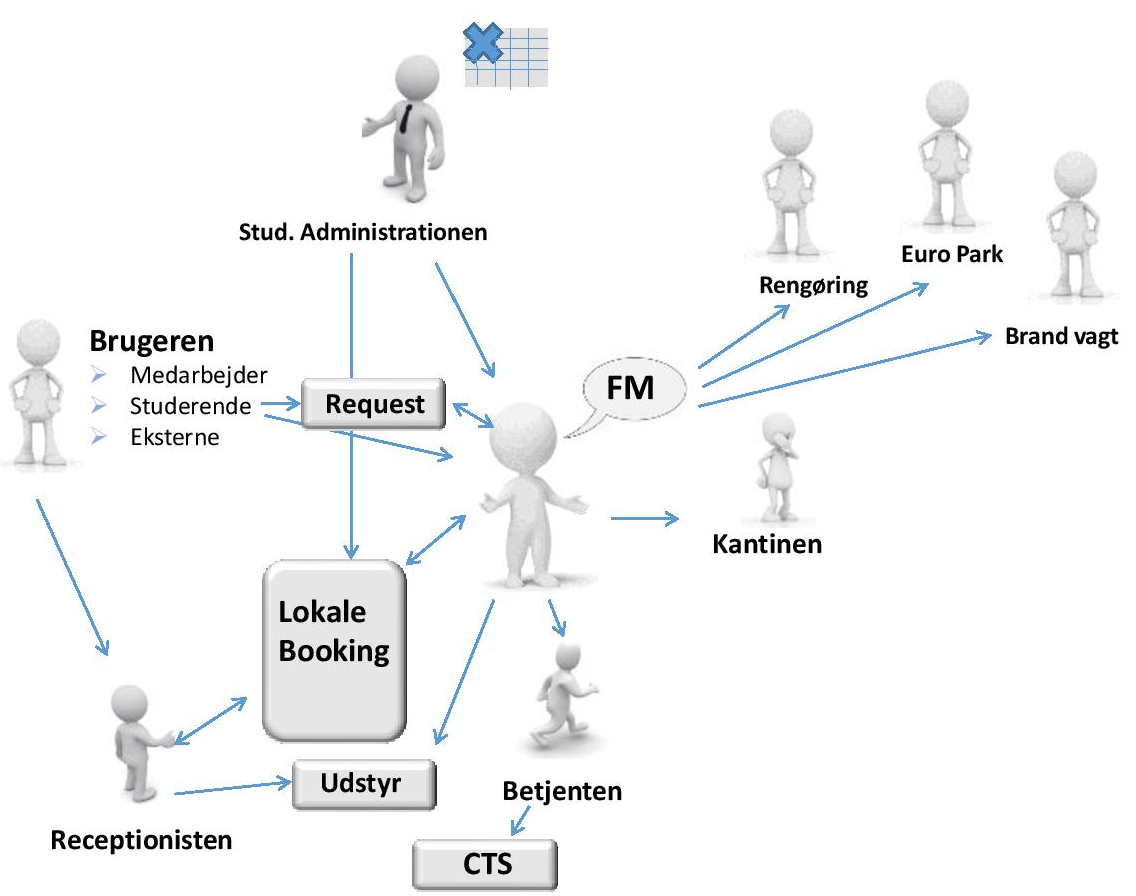
\includegraphics[width=0.5\textwidth]{Appendix/GUI-Prototype/NuvaerendeFlow}
  \caption{Nuværende system flow for booking systemet på ITU}
\label{Baggrund_kravspecifikationen_NuvaerendeFlow}
\end{figure}

\subsection{Ændringer til kravspecifikationen}
\label{Baggrund_kravspecifikationen_Aendringer}
Kravspecifikationen præsenterer en datamodel, der beskriver hvilke informationer systemet skal bruge. Vi har lavet nogle ændringer så den passer til vores implementering af bookingsystemet. Vi har fjernet lokale status og lavet en ”mange til én” forbindelse mellem booking og lokale da vi gerne ville have at en booking kun kunne have et lokale. Vi fjernede også "Lokale egenskaber" da vi vurderede, at det gav mest mening hvis "Inventar" repræsenterede et unikt stykke inventar og ikke havde antal i "Lokale egenskaber". Vi slettede også alle ”pris” værdier fra modellen, da vi ikke havde nogen intention om at understøtte fakturering.
\section{Arbejdsopgaver}
\label{Baggrund_Arb_opgaver}
Denne sektion beskriver hvilke arbejdsopgaver vi understøtter i første release samt giver en prioritering af, hvilke arbejdsopgaver der bør fokuseres på i følgende releases.
\subsection{Arbejdsområde 1: Booking}
\label{Baggrund_Arb_opgaver_Booking}
\subsubsection{C1: Administrer booking}
\begin{tabular}{ | l | r | p{5} |}
	\hline
	Arbejdesopgave & \\ 
\hline
	C1.1 & Understøttet \\ 
\hline
	C1.1a & Understøttet \\ 
\hline
	C1.2 & Understøtet \\ 
\hline
	C1.2a & Understøttet \\ 
\hline
	C1.3 & Understøttet \\ 
\hline
	C1.4 & Understøttet \\ 
\hline
	C1.5 & Understøttet \\ 
\hline
\end{tabular}

\subsubsection{C2: Forespørg på booking}
\begin{tabular}{ | l | r | p{5} |}
	\hline
	Arbejdesopgave & \\ 
\hline
	C2.1 & Understøttet \\ 
\hline
	C2.1a & Understøttet \\ 
\hline
	C2.2 & Understøttet \\ 
\hline
	C2.3 & Understøttet \\ 
\hline
\end{tabular}

\subsection{Arbejdsområde 2: Booking behandling}
\label{Baggrund_Arb_opgaver_Booking_behandling}
\subsubsection{C3: Modtag forespørgsel fra Eksern}
\begin{tabular}{ | l | r | p{5} |}
	\hline
	Arbejdesopgave & \\ 
\hline
	C3.1 & Understøttet \\ 
\hline
	C3.2 & Understøttet \\ 
\hline
	C3.2a & Understøttet \\ 
\hline
	C3.3 & Ikke understøttet \\ 
\hline
	C3.4 & Understøttet \\ 
\hline
	C3.5 & Understøttet \\ 
\hline
	C3.6 & Ikke understøttet \\ 
\hline
\end{tabular}

\subsubsection{C4: Klargør lokaler}
\begin{tabular}{ | l | r | p{5} |}
	\hline
	Arbejdesopgave &\\ 
\hline
	C4.1 & Ikke understøttet \\ 
\hline
	C4.2 & Ikke understøttet \\ 
\hline
	C4.3 & Ikke understøttet \\ 
\hline
\end{tabular}

\subsubsection{C5: Udlever nøgle}
\begin{tabular}{ | l | r | p{5} |}
	\hline
	Arbejdesopgave & \\ 
\hline
	C5.1 & Ikke understøttet \\ 
\hline
	C5.2 & Ikke understøttet \\ 
\hline
\end{tabular}

\subsection{Arbejdsområde 3: Forplejning}
\label{Baggrund_Arb_opgaver_Forplejning}
\subsubsection{C6: Håndter forplejning}
\begin{tabular}{ | l | r | p{5} |}
	\hline
	Arbejdesopgave & \\ 
\hline
	C6.1 & Ikke understøttet \\ 
\hline
	C6.2 & Ikke understøttet \\ 
\hline
	C6.3 & Ikke understøttet \\ 
\hline
	C6.4 & Ikke understøttet \\ 
\hline
\end{tabular}

\subsubsection{C7: Fakturer forplejning}
\begin{tabular}{ | l | r | p{5} |}
	\hline
	Arbejdesopgave & \\ 
\hline
	C7.1 & Ikke understøttet \\ 
\hline
	C7.5 & Ikke understøttet \\ 
\hline
\end{tabular}

\subsubsection{C8: Opadter menukort}
\begin{tabular}{ | l | r | p{5} |}
	\hline
	Arbejdesopgave & \\ 
\hline
	C8.1 & Ikke understøttet \\ 
\hline
\end{tabular}

\subsection{Arbejdsområde 3: Systemadministration}
\label{Baggrund_Arb_opgaver_Systemadmin}
\subsubsection{C9: Opdater listen for ekstra udstyr}
\begin{tabular}{ | l | r | p{5} |}
	\hline
	Arbejdesopgave & \\ 
\hline
	C9.1 & Understøttet \\ 
\hline
\end{tabular}

\subsubsection{C10: Opdater lokaler}
\begin{tabular}{ | l | r | p{5} |}
	\hline
	Arbejdesopgave & \\ 
\hline
	C10.1 & Understøttet \\ 
\hline
	C10.2 & Understøttet \\ 
\hline
\end{tabular}

\subsubsection{C11: Administrer bruger}
\begin{tabular}{ | l | r | p{5} |}
	\hline
	Arbejdesopgave & \\ 
\hline
	C11.1 & Ikke understøttet \\ 
\hline
	C11.1a & Ikke understøttet \\ 
\hline
\end{tabular}

\subsubsection{C12: Håndter statistik}
\begin{tabular}{ | l | r | p{5} |}
	\hline
	Arbejdesopgave & \\ 
\hline
	C12.1 & Ikke understøttet \\ 
\hline
	C12.2 & Ikke understøttet \\ 
\hline
\end{tabular}

\subsection{Arbejdsområde 4: Finans}
\label{Baggrund_Arb_opgaver_Finas}
\subsubsection{C13: Behandel faktura}
\begin{tabular}{ | l | r | p{5} |}
	\hline
	Arbejdesopgave & \\ 
\hline
	C13.1 & Ikke understøttet \\ 
\hline
	C13.2 & Ikke understøttet \\ 
\hline
\end{tabular}
\subsection{Prioritering af arbejdsopgaver}
\label{Baggrund_Arb_opgaver_Prio_Arb_Opg}
Til den første release af systemet valgte vi at fokusere på at understøtte systemadministration og booking af lokaler og udstyr, hvilket tydeligt kan ses i afsnit\ref{Arb_opgaver} da alle arbejdsopgaver i arbejdsområderne C1,C2,C3,C9 og C10 er understøttet. I kravspecifikationen er de arbejdsområder også blandt dem som er vægtet højest og det er samtidig de arbejdsområder som indeholder kernefunktionerne i systemet. Det som ikke blev prioriteret højt nok til at komme med i første release var de arbejdsopgaver som fokuserede på integrationen med kantinen, arbejdsopgaverne C6.1- C6.4 er eksempler på sådanne opgaver.
\\Grunden til at vi ikke tog de arbejdsopgaver med var, at vi vurderede, at de ikke var nødvendige for at have et system der understøttede basis funktioner, derudover lagde arbejdsopgaverne op til, at der skulle implementeres et interface specifikt til kantinen hvilket vi vurderede ville tage lang tid at implementere og vi ville også have tre brugergrupper at tage hensyn til ift. usability og testing.
Fokus for næste release vil derfor være at få udarbejdet et interface som kantinen kan bruge til at integrere med resten af systemet og få finpudset de allerede eksisterende funktioner, i kravspecifikationen. Behandling af faktura har også en høj vægtning så det vil der også være fokus på. 
\chapter{Design af brugergrænsefladen}
\label{Design_G}
Dette kapitel beskriver det generelle design af brugergrænsefladen samt de beslutninger, som ligger bag.

\section{Generelle mål}
\label{Design_G_Goals}
Vi har valgt at designe vores brugergrænseflade ud fra reglerne om design af virtuelle vinduer\cite[s. 169]{SL_UID} samt Ease Of Use principperne\cite[s. 9]{SL_UID}. I forbindelse med dette valg har vi sat følgende mål for designet:
\begin{itemize}
\item Strømlinet brugergrænseflade
\item Få forskellige skærmbilleder
\item Overblik
\item Effektivt
\end{itemize}

\subsection{Strømlinet brugergrænseflade}
Vi har valgt at designe skærmbillederne med samme grundstruktur. Denne lighed bør gøre det intuitivt at gå fra et skærmbillede til et andet i forbindelse med udførsel af opgaver. Desuden følger det designregel 1\footnote{Few window templates} om få vindueskabeloner.

\subsection{Kort vej fra en opgave til en anden}
Brugergrænsefladen skal gøre det hurtigt og nemt for brugeren at komme fra en opgave til en anden. Dette skal gøres ved at have få skærmbilleder involvereret i en enkelt task (designregel 2\footnote{Few window instances per task.}).

\subsection{Overblik}
Brugeren skal have mulighed for nemt at danne sig overblik over bookinger, udstyr og forplejning (regel 6\footnote{Necessary overview of data}). Derfor skal vi have seperate skærmbilleder, som giver overblik over hver type.

\subsection{Effektivt}
Det skal være effektivt at udføre opgaver for brugere, som anvender systemet ofte.

\section{Brugergrænsefladens udvikling og udseende}
\label{Design_G_Development}
Vores skærmbilleder er opdelt i tre typer: Gitter, Almindelig og Pop-ups. 
\\Gitterskærmbillederne bruger vi til booking af lokale, forplejning og udstyr samt administration af udstyr og lokaleinventar.
\\Almindelige vinduer anvender vi, hvis man skal ændre noget på et stykke udstyr/inventar eller et lokale.
\\Pop-up skærmbilleder er generelt advarsler eller fejlbeskeder.

For at få et overblik over hvordan man navigere i brugergrænsefladen og hvordan de forskellige skærmbilleder er designet, vil vi tage udgangspunkt i et eksemepel på hvordan work flowet for, hvis man skulle booke et lokale og tilføje forplejning til det. Vi vil derefter gennemgå de resterende interessante skærmbilleder individuelt.

Det første skærmbillede som man blive præsenteret for når man starter programmet er \ref{Design_G_Development_FinalGrid} her man i stand til at markere de tider man gerne vil booke et lokale, for at kunne booke skal man dog først logge ind via login knappen i øverste højre hjørne. 

Vores første mockup af gitterskærmbilledet se figur \ref{Design_G_Development_FirstGrid} havde et gitter, hvor hver række var et lokale og tiderne var kolonner. Man skulle klikke i et felt for at vise, at man ønskede at booke på et bestemt tidspunkt. Når man havde valgt de tider og lokaler, man gerne ville booke, skulle man trykke på en "Book" knap. 
Som man kan se på Figur \ref{Design_G_Development_FinalGrid} valgte vi at beholde den struktur, men vi tilføjede checkboxses til gitteret. Dette blev gjort efter første runde af usability tests hvor vi observerede, at brugeren var i tvivl om, hvor man skulle klikke for at vælge tider for en booking, derudover tilføjede vi også, at udstyr m.m., man har booket, ligger øverst i gitteret, når man får oversigten over fx udstyr. Dette gør det nemt at finde det element, man har booket/bestilt.

\begin{figure}[h!]
  \centering
    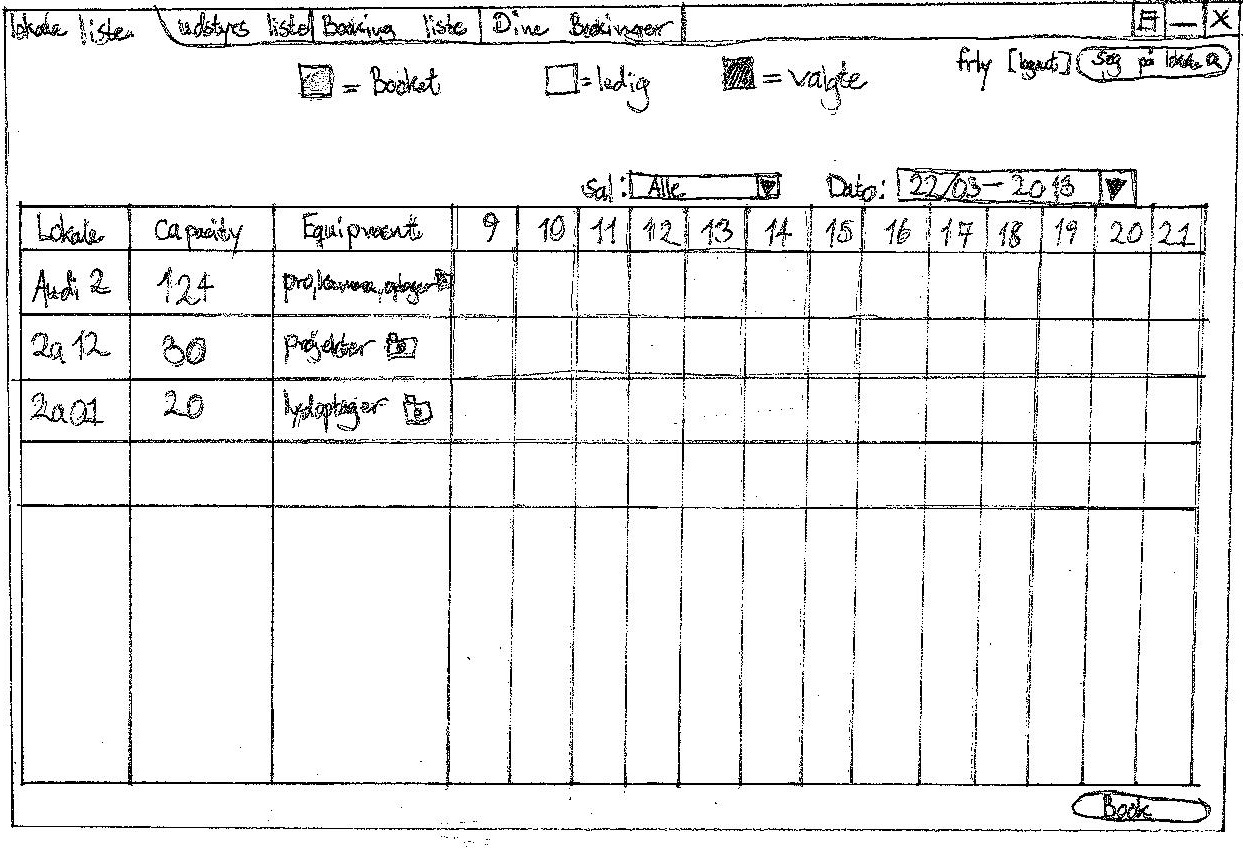
\includegraphics[width=0.5\textwidth, angle=90]{Appendix/GUI-Prototype/PaperMockup/LokaleListe_001}
  \caption{Første udgave af gitter layoutet}
\label{Design_G_Development_FirstGrid}
\end{figure}

\begin{figure}[h!]
  \centering
    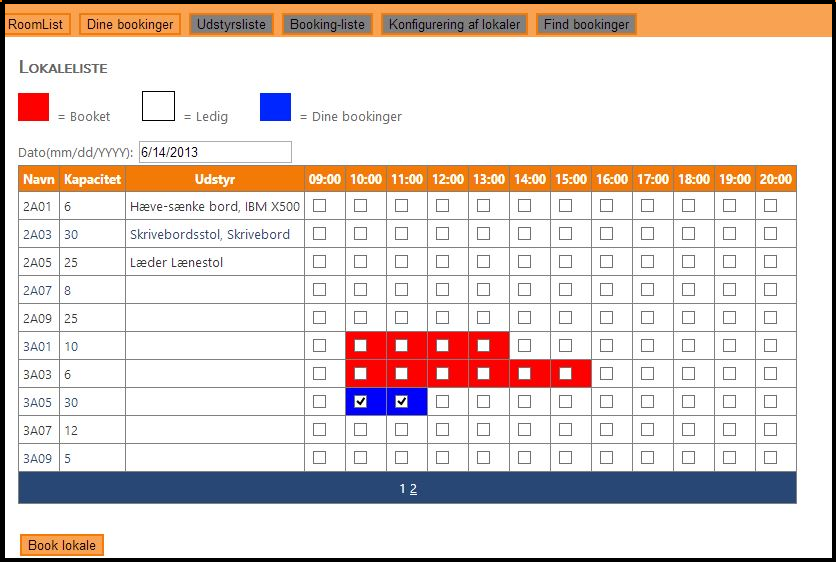
\includegraphics[width=0.5\textwidth]{Appendix/GUI-Prototype/DigitalMockup/GridEksempel}
  \caption{Den endelige udgave af gitteret}
\label{Design_G_Development_FinalGrid}
\end{figure}

Hvis man markere et lokale i det tidsrum man gerne vil booke det og trykker book vil bookingen blive oprettet og man vil blive navigeret videre til en side der visser en oversigt over alle dine bookinger, se figur\ref{Design_G_Development_YourBookings_Final}. 

Til designet af det skærmbillede fokuserede vi på at overholde Gestalt-lovene\cite[s. 68]{SL_UID}, specifikt Law of Proximity\footnote{"Pieces that are close together are perceived as belonging together".}, da vi gerne ville opnå, at det virkede intuitivt for brugeren, at det var de knapper der skulle bruges til at interegere med gitteret. 

\begin{figure}[h!]
  \centering
    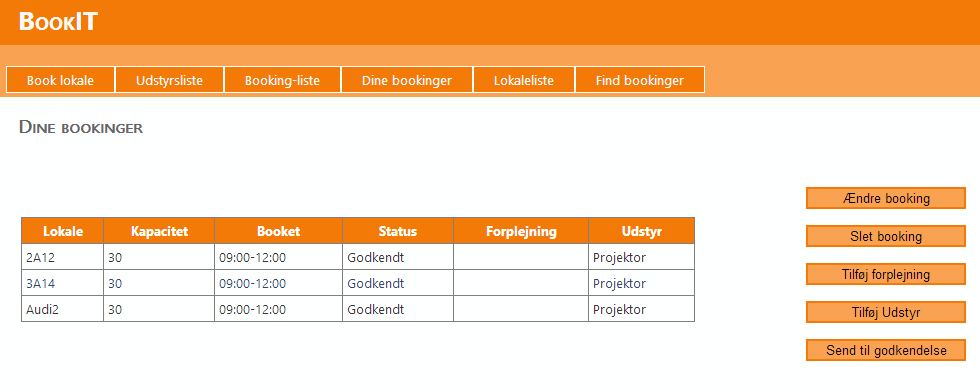
\includegraphics[width=0.5\textwidth]{Appendix/GUI-Prototype/DigitalMockup/DineBookinger}
  \caption{Skærmbilledet til visning af bookinger}
\label{Design_G_Development_YourBookings_Final}
\end{figure} 

Figur\ref{Design_G_Development_Forplejning_Final} viser det endelige skærmbilled til forplejnings valg. Til designet af skærmbillede fokuserede vi på, at det grafisk skulle minde om \ref{Design_G_Development_FinalGrid således, at vi overholdte designregel 1 på den måde ville brugeren intuitivt vide hvordan man skulle tilføje forplejning. De samme design beslutninger gælder for tilføjelse af udstyr til en booking, skærmbilledet kan ses i  \ref{Appendix} på side \pageref{Appendix}.

\begin{comment}
\begin{figure}[h!]
  \centering
    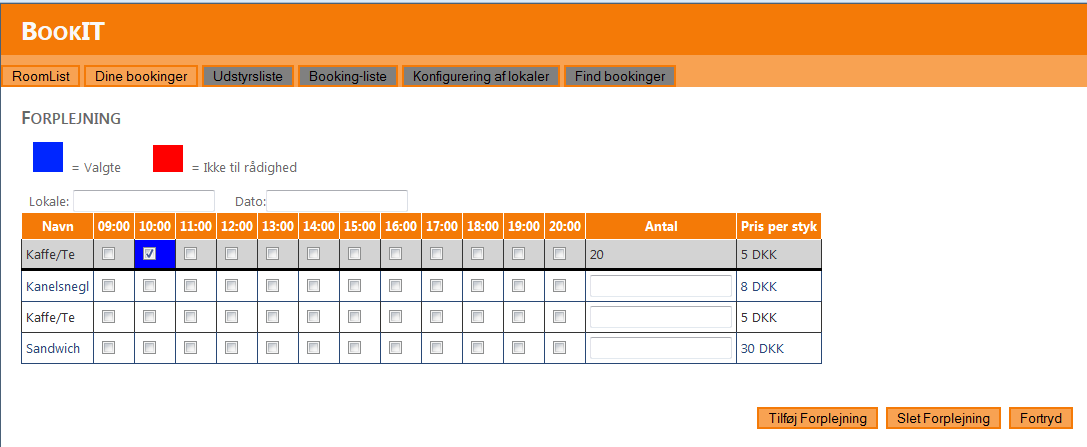
\includegraphics[width=0.5\textwidth]{Appendix/GUI-Prototype/DigitalMockup/Forplejning}
  \caption{Skærmbilledet til booking af forplejning}
\label{Design_G_Development_Forplejning_Final}
\end{figure} 
\end{comment}
\subsection{Bookingliste}
For at en bruger kan tilføje udstyr eller forplejning til sin booking skal den først godkendes. Dette gøres af recepsionisten, som har en liste over alle bookinger som brugerne har oprettet, se figur \ref{Design_G_Development_BookingListe_Final}. Til det endelig design af skærmbilledet valgt vi at flytte godkend/afvis knapperne fra inde i gitteret, som de var i papermockupen se figur \ref{Design_G_Development_BookingListe}, til at være ved siden af gitteret således at vi ligesom i figur\ref{Design_G_Development_YourBookings_Final} benyttede "Law of proximity". Desuden havde ingen af de andre gittre knapper i sig, så vi vurderede, at det så vidt muligt skulle være ens på alle billeder således, at vi overholdt designregel 1.

\begin{comment}
\begin{figure}[h!]
  \centering
    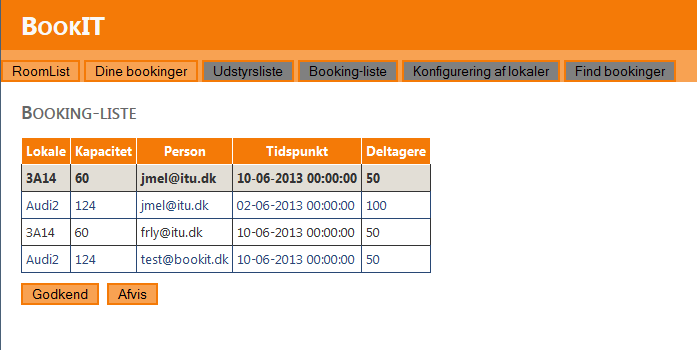
\includegraphics[width=0.5\textwidth]{Appendix/GUI-Prototype/DigitalMockup/BookingListe}
  \caption{Skærmbilledet af recepsionistens liste af bruger bookinger.}
\label{Design_G_Development_BookingListe_Final}
\end{figure} 
\end{comment}

\begin{figure}[h!]
  \centering
    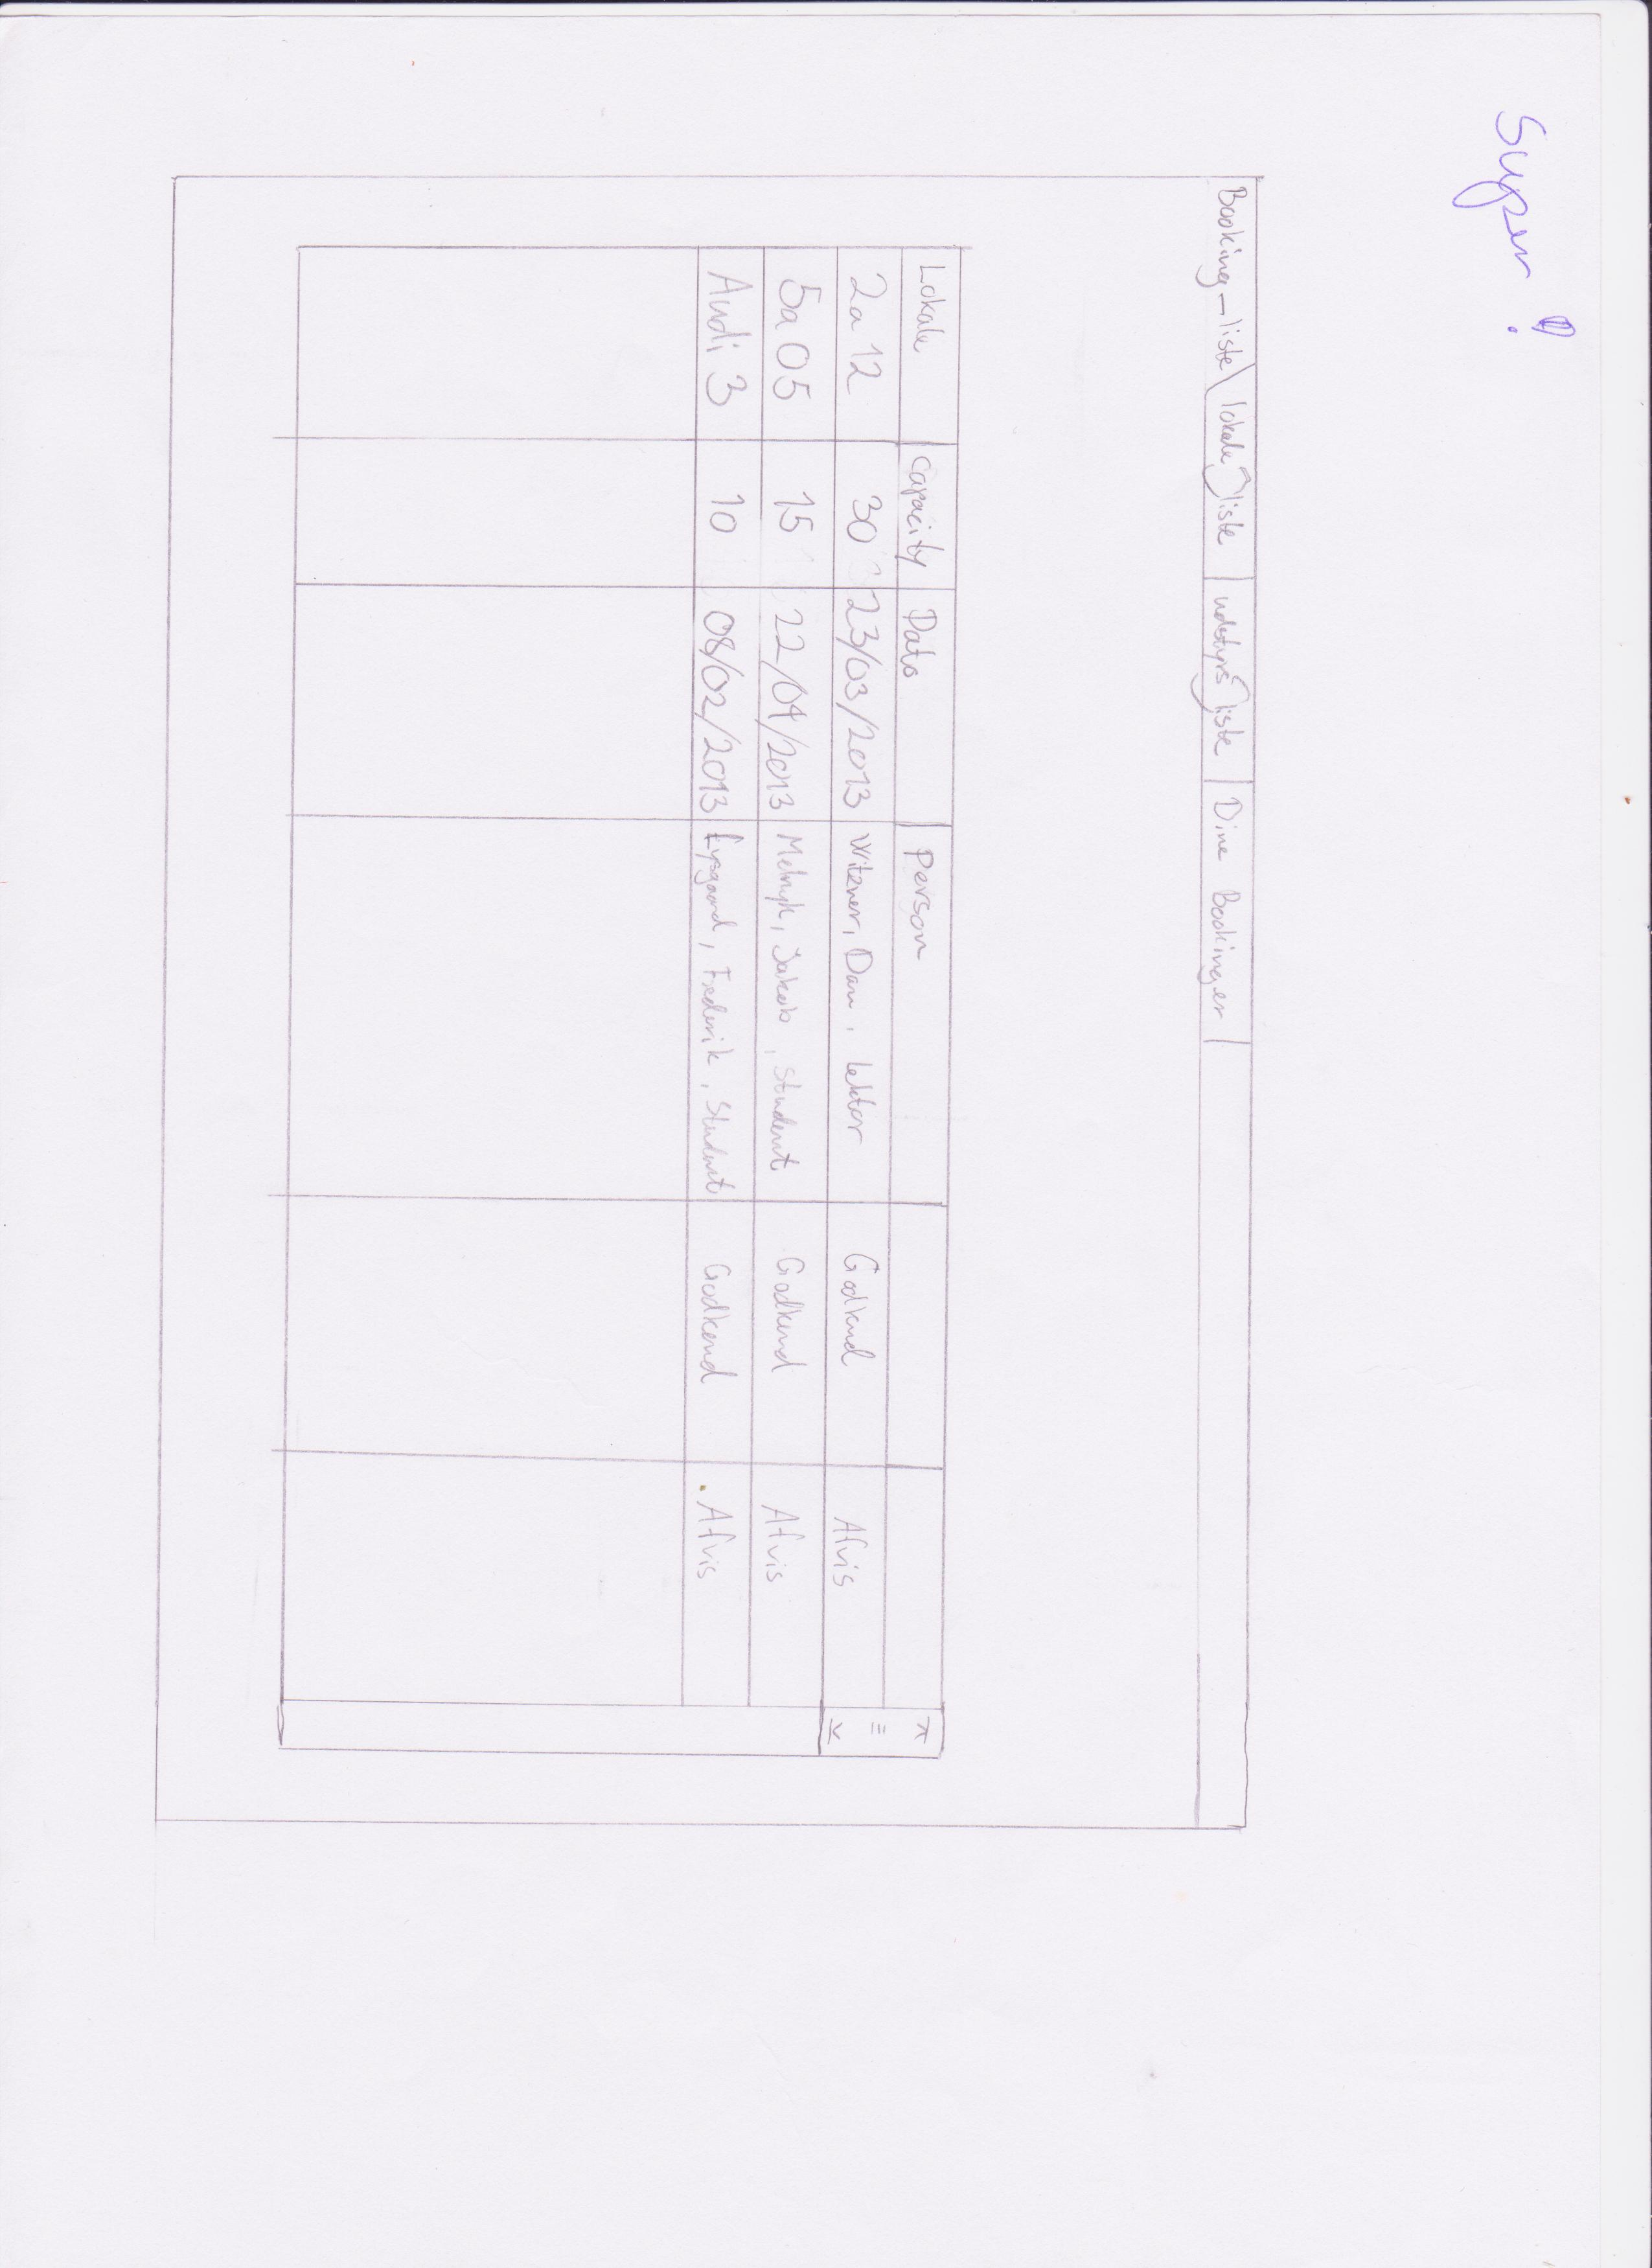
\includegraphics[width=0.5\textwidth]{Appendix/GUI-Prototype/PaperMockup/GodkendBookinger_001}
  \caption{Papermockup af recepsionistens liste af bruger bookinger.}
\label{Design_G_Development_BookingListe}
\end{figure} 

\subsection{Udstyrsliste}
Figuren \ref{Design_G_Development_BookingListe_Final} viser det endelige skærmbillede af listen over udstyr og tilføjelse af nyt udstyr til systemet. Til designet af skærmbilledet brugte vi "Law of proximity" så det er tydeligt, at de to funktionaliteter i skærmbilledet ikke hører sammen. Den eneste ændring der er blevet lavet til det endelige skærmbillede  i forhold til den originale papermockup\ref{Appendix} på side \pageref{Appendix} er, at der er blevet tilføjet en checkbox, hvor man kan vælge om udstyret skal kunne udlånes. Hvis den ikke udfyldes vil udstyret blive kvalificeret som inventar og det vil derfor ikke blive vist under muligt udstyr, der kan tilføjes en booking. 

\begin{comment}
\begin{figure}[h!]
  \centering
    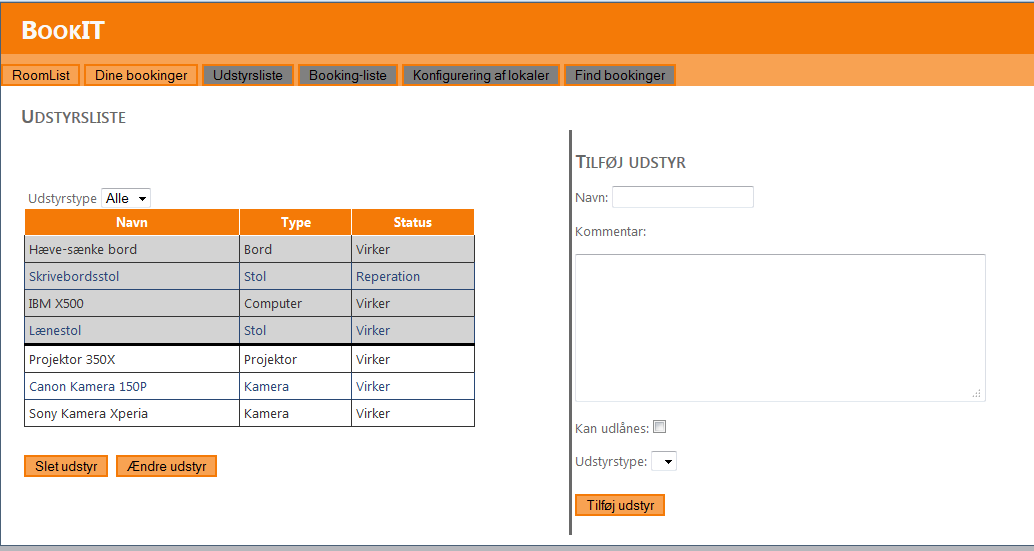
\includegraphics[width=0.5\textwidth]{Appendix/GUI-Prototype/DigitalMockup/UdstyrsListe}
  \caption{Skærmbilledet af recepsionistens liste over udstyr i ITUs system.}
\label{Design_G_Development_UdstyrsListe_Final}
\end{figure} 
\end{comment}

\subsection{Lokale liste}
I systemet er der også mulighed for ændre i listen over lokaler, se figur \ref{Design_G_Development_LokaleListe_Final}. Til designet af skærmbilledet fokuserede vi på, at der skulle være klart overblik, vi sørgede derfor for at overholde law of proximity ved at ligge knapperne tæt på gitteret, hvilket også gør, at det kun er det vigtige information der bliver præsenteret i gitteret.

\begin{comment}
\begin{figure}[h!]
  \centering
    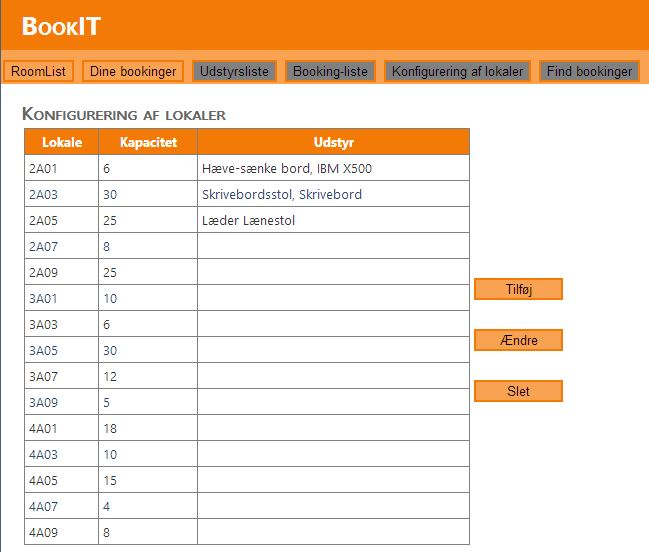
\includegraphics[width=0.5\textwidth]{Appendix/GUI-Prototype/DigitalMockup/LokaleListe}
  \caption{Skærmbilledet af recepsionistens liste over lokaler i ITUs system.}
\label{Design_G_Development_LokaleListe_Final}
\end{figure} 
\end{comment}

\subsection{Ændring af lokale}
Til ændring af lokaler i systemet fokuserede vi på, at man skulle være i stand til at ændre de basale ting som navn og kapacitet, og samtidig være i stand til, at se en liste over inventar i lokalet hvor man skulle kunne tilføje eller fjerne udstyr. Til papermockupen, se figur \ref{Design_G_Development_AendreLokale} havde vi skærmbilledet opdelt i tre afsnit, et til at skifte kapcitet og navn, et til at tilføje inventar og et til at slette inventar.

Dette var en meget uoverskuelige løsning og den var ikke strømlignet i forhold til resten af GUI'en. Vi valgte at lave en løsningen som var i stil med de andre skærmbilleder se figur \ref{Design_G_Development_AendreLokale_Final} vi valgte, at skærmbilledet kun skulle være fokuseret på en gitterløsning hvor den øverste del ville være det udstyr der allerede var i lokalet og resten af gitteret ville så være fyldt med udstyr som man kunne vælge at tilføje til lokalet.

\begin{comment}
\begin{figure}[h!]
  \centering
    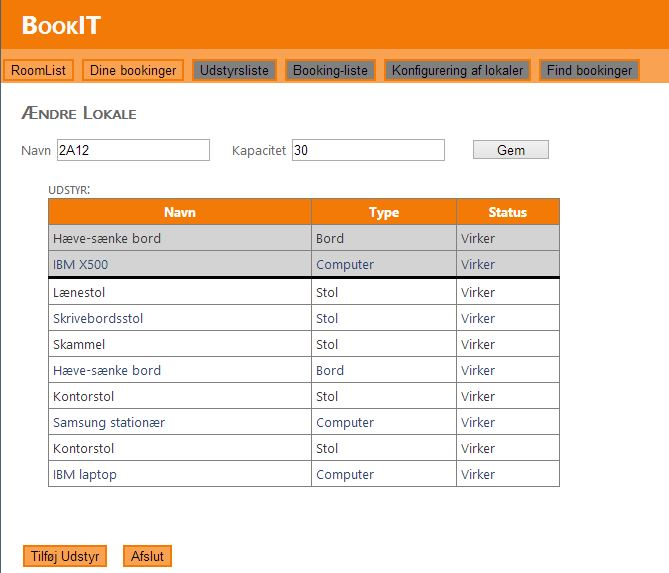
\includegraphics[width=0.5\textwidth]{Appendix/GUI-Prototype/DigitalMockup/AendreLokale}
  \caption{Skærmbilledet til ændring af lokale.}
\label{Design_G_Development_AendreLokale_Final}
\end{figure} 
\end{comment}

\begin{figure}[h!]
  \centering
    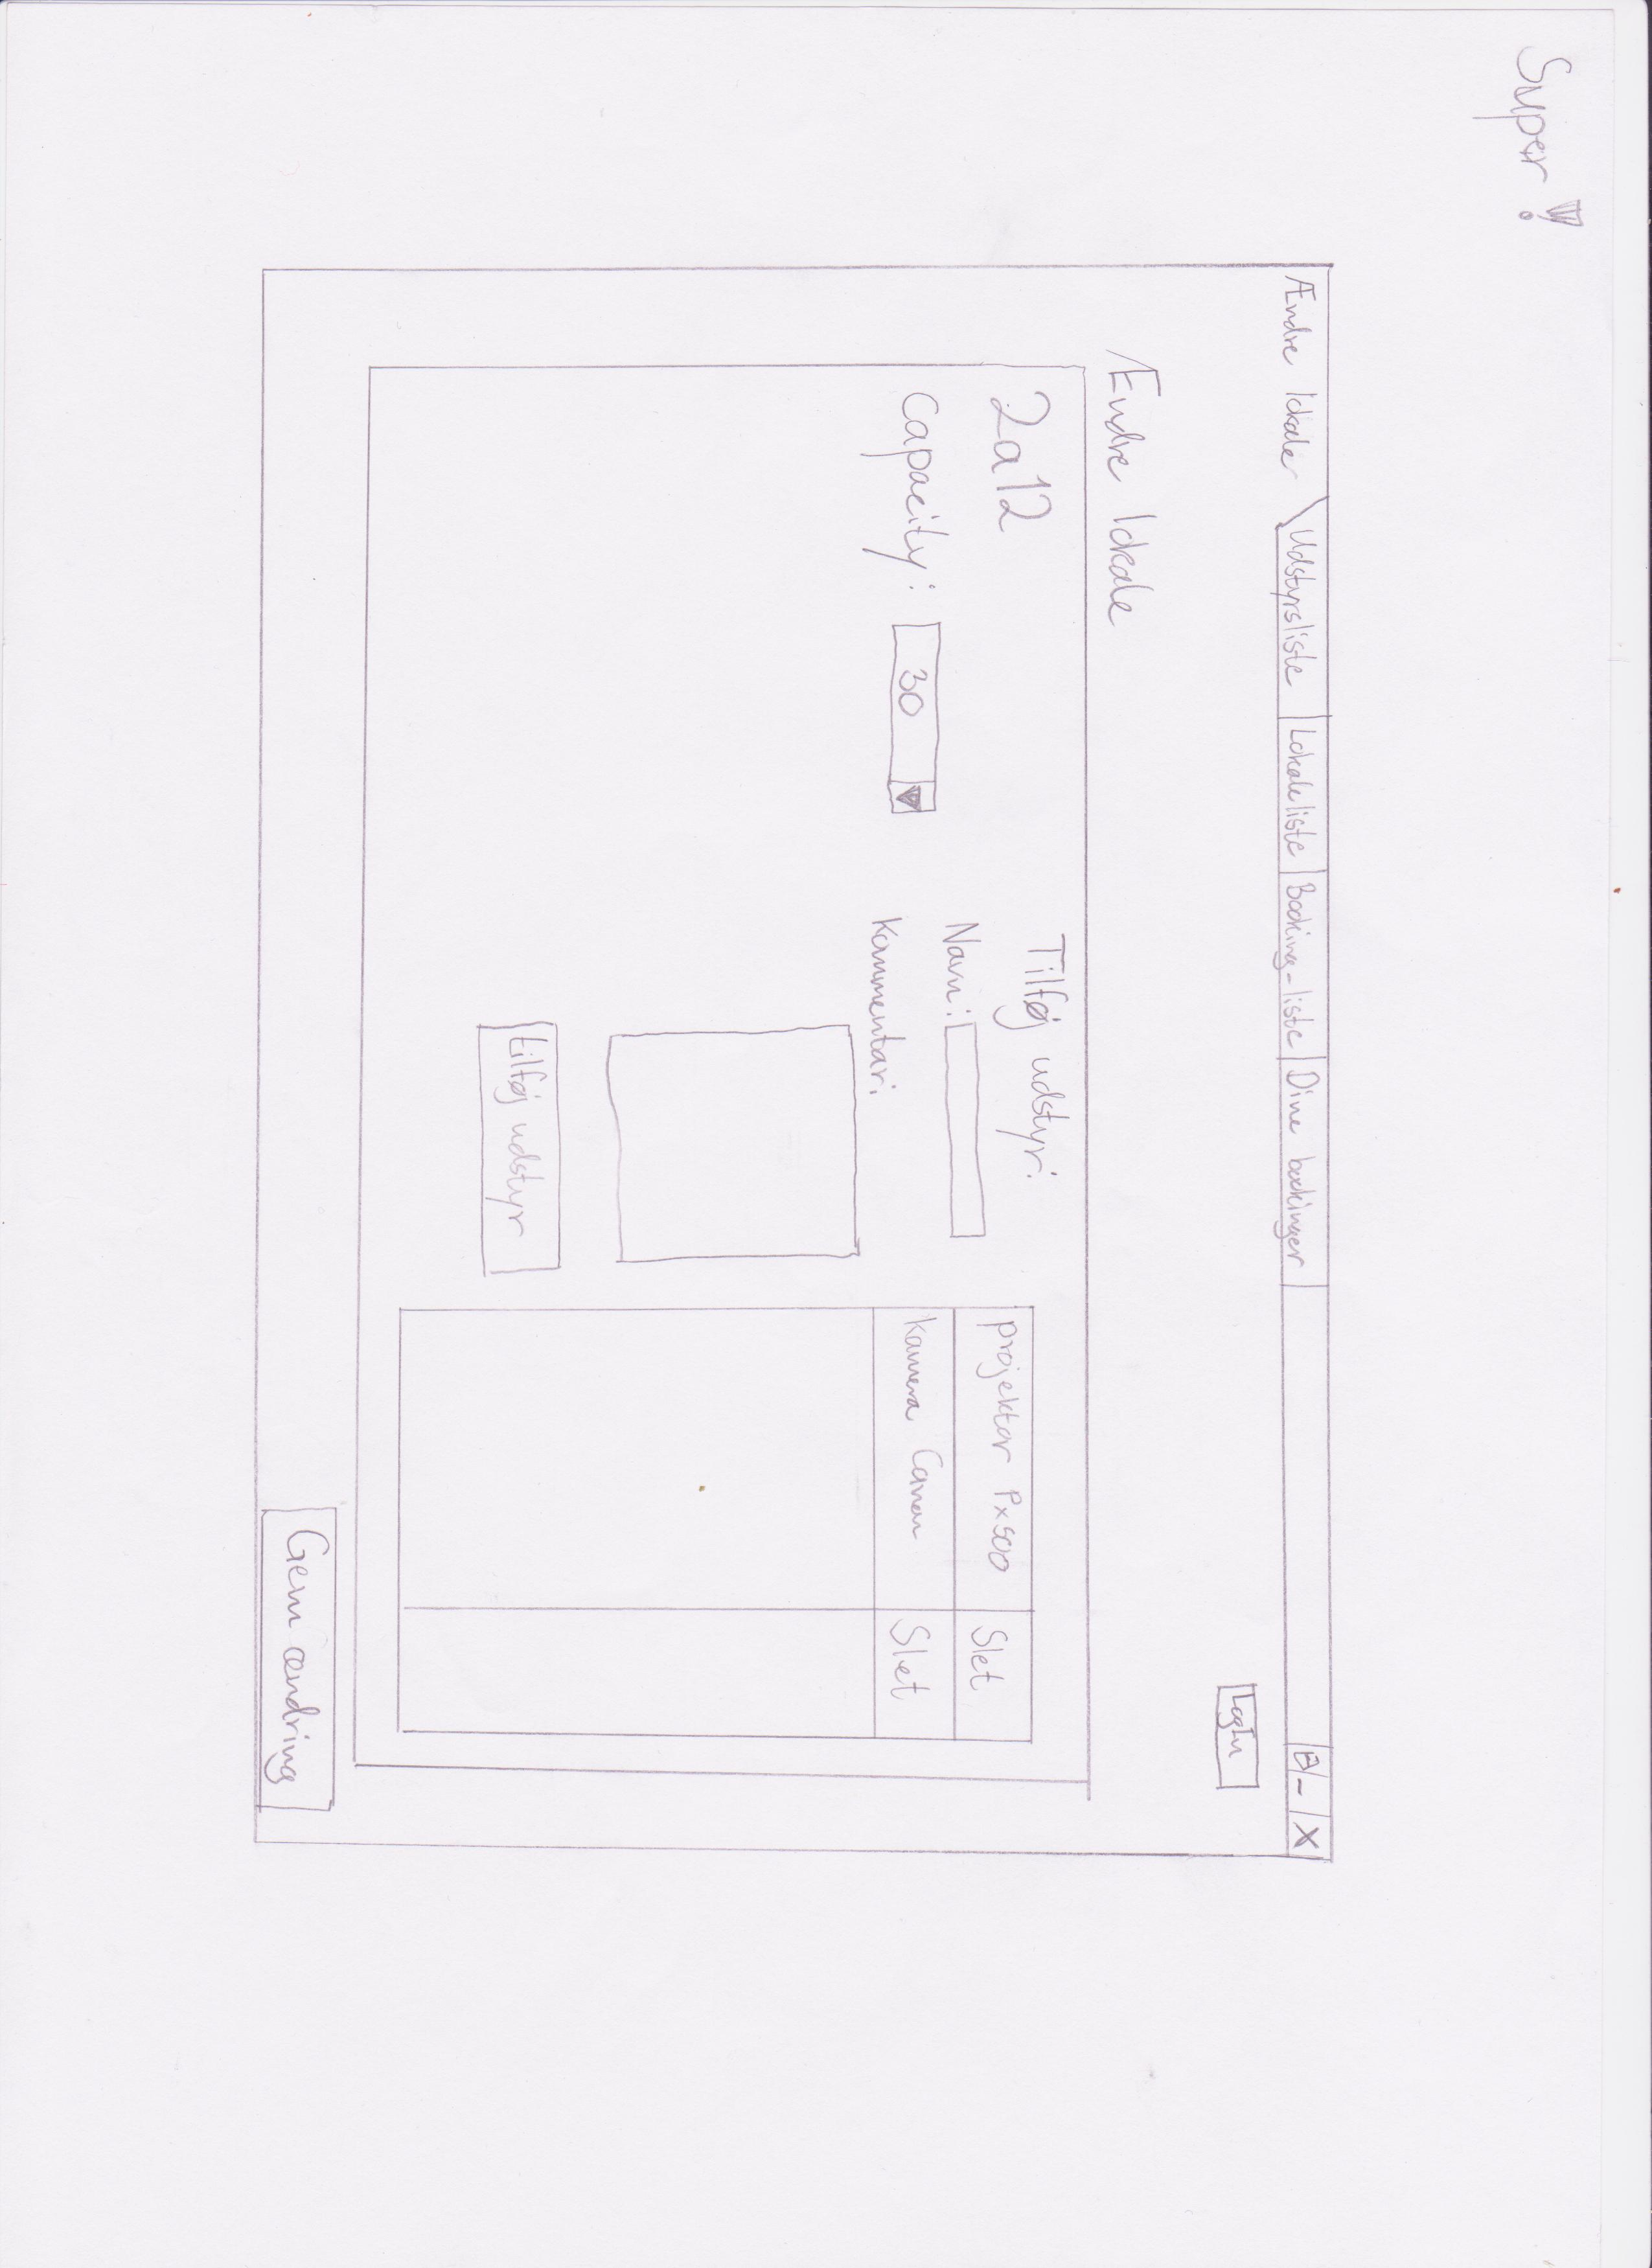
\includegraphics[width=0.5\textwidth]{Appendix/GUI-Prototype/PaperMockup/AendreLokale_001}
  \caption{Papermockup til ændring af lokale.}
\label{Design_G_Development_AendreLokale}
\end{figure} 
\chapter{Usability testing}
\label{Usability}
Dette kapitel beskriver, hvad vores strategi for usability testing har været samt resultaterne af vores tests.

\section{Test strategi}
\label{Usability_TS}
Kravspecifikationen beskriver, at det er nødvendigt at lave usability tests tidligt i processen for at bevise proof of concept. Vi lavede papermockups af vores skærmbilleder for at opfylde dette krav. 

Vi valgte at lave to runder af usability tests.
\\Runde 1 bestod af tests med en papermockup på en enkelt bruger.
\\Runde 2 bestod af tests af det endelige produkt på flere brugere.

Vi valgte kun at teste én bruger i runde 1, da flere testpersoner tidligt i udviklingsfasen kan føre til en overvældende liste af problemer\cite[s. 416]{SL_UID}. Derudover er en enkelt testperson ofte nok til at afsløre de mest seriøse problemer i brugergrænsefladen.

Vi mener, at det havde været optimalt, hvis vi kunne have udført en usability test midtvejs i processen (mellem runde 1 og runde 2), men vi vurderede, at vi ikke ville få nok ud af testen, da det ville være svært at finde tid til at teste nok personer samt implementere de mulige ændringsforslag.

\subsection{Test cases}
\label{Usability_TS_TC}
Vi har to brugergrupper i vores usability tests. Der er almindelige brugere (studerende/undervisere) og administration (Facility Management/Receptionister). Til hver af disse brugergrupper har vi defineret syv test cases.

Test cases til almindelige brugere:
\begin{description}
\item[Test Case 1:] Du har booket et lokale fra 9-10 til et møde med din vejleder og du vil gerne have en diktafon med, så du kan optage mødet.
\item[Test Case 2:] Du skal holde et møde på tre timer om et par dage. Du skal i den sammenhæng booke et lokale til formålet.
\item[Test Case 3:] Et af dine gruppemedlemmer har meldt tilbage, at han skal aflevere sin datter i børnehaven. Mødet kan derfor først holdes fra klokken 10.
\item[Test Case 4:] Da mødet ligger om morgen, tænker du, at det vil være fornuftigt, hvis der var noget kaffe og morgenbrød klar.
\item[Test Case 5:] Du skal til dit projekt optage en kort reklamefilm og har derfor brug for et kamera.
\item[Test Case 6:] Et af dine gruppemedlemmer har kamera med, så du behøver ikke længere booke et hos ITU.
\item[Test Case 7:] Deltagerne til dit møde i 2a12 har desværre aflyst.
\end{description}
Test cases til administrationsbrugere:
\begin{description}
\item[Test Case 1:] En elev har kontaktet dig og gjort dig opmærksom på, at der ikke længere er en projektor i 2A12.
\item[Test Case 2:] ITU har til sin udstyrssamling erhvervet sig to nye kameraer.
\item[Test Case 3:] En student henvender sig til dig ved skranken og spørger om hans booking er blevet godkendt.
\item[Test Case 4:] Du har et møde  i de kommende dage og vil helst gerne holde det på 4. sal.
\item[Test Case 5:] Du skal afholde et fordrag for 30 mennesker den 24, tidspunktet er irelevant men der skal være plads til min. 30 mennesker.
\item[Test Case 6:] Lokalet 5a12 er ikke længere et privat lokale, men skal istedet registreres som et mødelokale.
\item[Test Case 7:] Lokalet 2a12 er ikke længere til rådighed i forbindelse med booking.
\end{description}

Vi har designet vores test cases således, at testpersonen ikke får at vide hvor i systemet, de skal udføre deres arbejdsopgave. Dette har vi gjort for at finde ud af, hvor intuitivt vores system er.
\\De 14 test dækker til sammen størstedelen af systemets workflows. Vi udfører testene som "think aloud" tests\cite[s. 421]{SL_UID}. "Think-aloud" tests består af at læse test casen op for testpersonen og bede dem tænke højt og forklare, hvad de gør under testen.

Efter testen får brugeren mulighed for at give input til, hvad de synes er godt og hvad der kan forbedres. Dette giver os mulighed for at få et indtryk af, hvad vi har overset i vores design og hvilke elementer, vi bør bruge flere steder i systemet.

I første runde af tests havde vi fokus på de store problemer i systemet, hvor vi i anden runde havde fokus på at følge op på de ændringer, vi havde lavet i forhold til resultaterne fra første runde. I anden runde var vi også interesserede i at finde ud af, om vores system er intuitivt og effektivt nok.

\section{Runde 1: Resultater og konsekvenser}
\label{Usability_R1}
Efter den første runde af tests var der fem problemer, problemerne er klassifikeret i forhold til skalaen fra \cite[s. 439]{SL_UID}:
\begin{description}
\item [Punkt 1:] Minor problem - Usikker på hvordan man vælger booking tidspunkter.
\item [Punkt 2:] Cumbersome - Brugeren synes det var besværlig at navigere imellem skærmbillederne.
\item [Punkt 3:] Medium problem - Svært ved at forstå sletning af forplejning/udstyr og booking.
\item [Punkt 4:] Minor problem - Problem med at tilføje udstyr/forplejning.
\item [Punkt 5:] Positiv feedback på den generelle struktur af systemet.
\end{description}

\paragraph{Punkt 1}
Test personen havde problemer med at finde ud af, hvordan vores gitter til booking af lokaler fungerede. Personen troede ikke, man kunne klikke på felterne i gitteret, så der skulle lidt hjælp til, før personen forstod princippet.
\subparagraph{Konsekvenser og løsning}
Vi blev enige om, at dette problem kunne løses ved at indsætte en checkbox i felterne. Det vil gøre det mere intuitivt, når man skal trykke på tiderne.

\paragraph{Punkt 2}
Testpersonen følte, at der manglede navigeringsmuligheder mellem de forskellige skærmbilleder. Det var ikke intuitivt, at man skulle bruges tabsne til at skifte skærmbillede.
\subparagraph{Konsekvenser og løsning}
Vi løste problemet ved at lave en menubar, som var placeret nærmere midten af billedet, så den blev mere synlig.

\paragraph{Punkt 3}
Testpersonen fandt det ikke naturligt, at man skulle bruge lokalelisten til at ændre sin booking.
\subparagraph{Konsekvenser og løsning}
Da det var første test af vores system og det kun var testet på en person valgte vi ikke at gøre noget ved problemet da vi mente, at vores grundstruktur i systemet var solid og derfor ikke burde ændres kun på grund af det problem.

\paragraph{Punkt 4}
Testpersonen nævnte, at hun ikke mente, det burde være muligt at tilføje udstyr/forplejning til en booking før, den er blevet godkendt.
\subparagraph{Konsekvenser og løsning}
Vi valgte at imødekomme dette ved at implementere logik, så man ikke kan trykke på knapperne til at tilføje forplejning/udstyr, hvis man ikke har valgt en godkendt booking.

\paragraph{Punkkt 5}
Testpersonen kunne godt lide den overordnede struktur af systemet og var positiv overfor booking funktionaliteten (gitteret). Personen skulle bare lære at bruge booking funktionaliteten.
\subparagraph{Konsekvenser og løsning}
Denne feedback havde stor indflydelse på, at vi valgte at beholde vores grundstruktur.

\section{Fremgangs måde for usabilitytest runde 2}
\label{Usability_R2}
Vi nåede desværre ikke at lave en anden runde af usabilitytests før produktet skulle aflevers, den sidste runde af usabilitytests vil derfor først blive lavet efter at produktet er færdigt. Vi vuderede dog stadig at det er i ITU's interesse, at der bliver lavet usabilitytests på det færdige system, for både at bevise brugervenligheden i systemt og finde eventuelle mangler og bugs. Måden hvorpå vi ville have foretaget anden runde af usabilitytest, ville være at vi tog to til tre test personer fra hver test gruppe, som vi ville lave "think-aloud" test på ligsom i første runde af tests, vi ville bruge de samme test cases som vi brugte i første runde af tests. Vi vil ligesom i første runde tag en snak med brugeren efter hver test for at høre hvad de synes om systemet og om de har ideer til mulige forbedringer.  

\section{Mulige konsekvenser af usabilitytest runde 2}
\label{Usability_R2_Possibilities}
Optimalt set ville konsekvenserne af den anden usabilitytest runde være, at der ikke er nogen af problemerne fra første runde der går igen, dette ville tyde på at det overordnet design er i orden og vi derfor vil være i stand til kun at fokusere på at forbedre funktionaliteten af programmet.
Det er dog mere realistisk at brugerne stadig vil synes at der er nogle mindre problemer med brugergrænsefladen, vi vil derefter vudere om hvorvidt der er nok bruger der synes det er et problem og om problemet kan klassificeres som noget der burde fikses. Hvis vi finder at alle brugerne støder på et problem og har besværligheder med færdiggøre en task, vil vi gør ITU opmærksom på fejlen og komme med en liste over mulige løsning forslag.
\chapter{Teknisk design}
\label{Technical}

\section{Cost/benefit analyse af arkitektur og platform}
\label{Technical_CostBen}
Da vi skulle implementere vores system var det vigtigt for os, at vi vælge den korrekte implementationsstrategi i forhold til, hvor meget gavn brugeren ville få ud af de forskellige løsninger. Vi overvejede derfor, hvor stor en nytteværdi det ville have for brugerne, hvis vi brugte en implementationsmulighed frem for en anden og hvor meget, det ville koste os at implementere den. 

Vi lavede et skema, som viser et overblik over vores cost-benefit analyse. \textcolor{red}{X} viser vores omkostning, \textcolor{Green}{O} viser nytteværdien for brugerne. Små bogstaver indikerer halve værdier.

\begin{table}[h]
\begin{centering}
\begin{tabular}{| r | c | c | c | c | c | c |}
\hline
 & Java & .Net & WCF (.Net) & Webserv. (Java) & Restful (.Net) & Restful (Java)\\
\hline
Thick browser klient & \textcolor{red}{XX} & \textcolor{red}{XX} & & & & \\ \cline{2-3}
 & \textcolor{Green}{O} & \textcolor{Green}{OO} & & & & \\
\hline
Thick application klient & \textcolor{red}{X} & \textcolor{red}{X} & & & & \\ \cline{2-3}
 & \textcolor{Green}{Oo} & \textcolor{Green}{O} & & & & \\
\hline
Webservice(browser) & & & \textcolor{red}{XXX} & \textcolor{red}{XXXX} & \textcolor{red}{XXXx} & \textcolor{red}{XXXX} \\ \cline{4-7}
 & & & \textcolor{Green}{OOOO} & \textcolor{Green}{OOO} & \textcolor{Green}{OOOO} & \textcolor{Green}{OOOo}\\
\hline
Webservice(application) & & & \textcolor{red}{XX} & \textcolor{red}{XXX} & \textcolor{red}{XXx} & \textcolor{red}{XXX} \\ \cline{4-7}
 & & & \textcolor{Green}{OOo} & \textcolor{Green}{OOOo} & \textcolor{Green}{OOO} & \textcolor{Green}{OOOO}\\
\hline
\end{tabular}
\end{centering}
\caption{Tabel over cost/benefit i forhold til de forskellige implementationsmuligheder}
\label{fig:Technical_CostBen_Table}
\end{table}

For at komme frem til omkostningerne af de forskellige implementationsmuligheder tog vi udgangspunkt i hvorvidt vi først skulle tilegne os viden eller om vi allerede havde den fornødende forståelse og således kunne gå i gang med det samme. eksempelvis ville en "Java, Thick browser client" løsning være dyrere end en "Java, Thick application client"løsning da vi ikke ved, hvordan man laver en browser klient i java. Derefter kiggede vi på, hvor meget kode der skulle skrives til de forskellige implementationsmodeller for at kunne få et fungerende system. Eksempelvis er alle Webservice løsningerne dyrere end Thick client løsningerne, da der skal kodes mere, hvis der skal laves en webservice.

En af måderne, vi fandt ud af hvor meget gavn de forskellige implementationsmuligheder gav brugeren var at se på, hvor mange platforme der var understøttet.
\\Eksmepelvis synes vi, at det gav brugeren mere nytte, hvis systemet kunne køre på alle computerere i en browser end, hvis man skulle downloade/installere en klient og tjekke, om den kunne køre på computeren.
\\Derudover kiggede vi også på, hvor nemt det ville være for brugeren at udvikle videre på systemet, eksempelvis giver implementationsmuligheden "WCF(.NET), Webservice(browser client)" brugeren mulighed for at udvikle en applikation til Windows Phone, da der er en service at kode op imod.

Udfra tabel \ref{fig:CostBen_Table} er der to valgmuligheder, som har det bedste forhold mellem benefit og omkostning. Både WCF webservice med en tilhørende browser klient og en Resful Java Webservice med en application klient har forholdet \begin{math}\frac{benefit}{cost} = \frac{4}{3} \sim 1.33333\end{math}. Vi valgte WCF løsningen på baggrund af, at det er en løsningstype, vi har erfaring med fra et tidligere projekt.
\\Det viste sig dog senere, at det slet ikke var nødvendigt at udvikle webservicen i forbindelse med første release. Det forlængede udviklingsprocessen, hvilket betød, at der var funktionalitet, vi ikke fik implementeret.

\section{Databasen}
\label{Technical_Database}

\subsection{Kravspecifikationens datamodel}
\label{Technical_Database_ks}
Kravspecifikationens kapitel \textit{D} \cite[s.14]{kravspec} præsenterer følgende model for det data, systemet skal bruge:
\begin{figure}[h!]
  \centering
    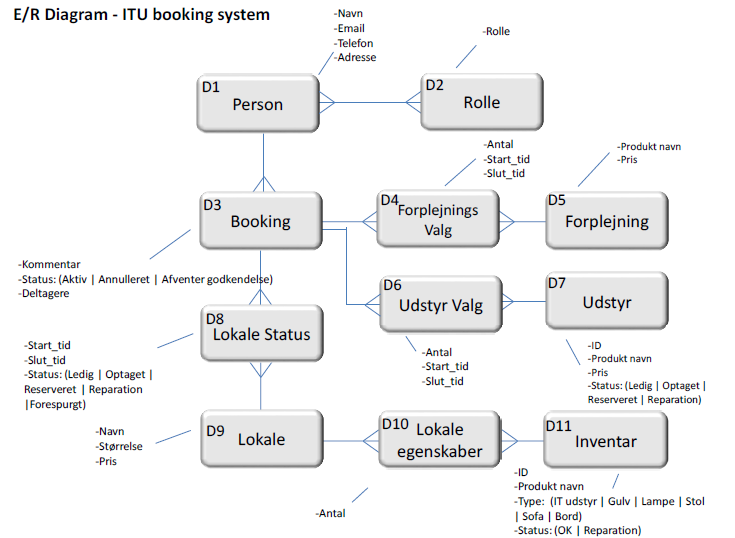
\includegraphics[width=\textwidth]{Chapters/Design/Technical/Images/KSdata}
  \caption{Kravspecifikationens datamodel}
\label{Fig:Technical_Database_ks_KSdata}
\end{figure}

Der er en række ting, som skal ændres ved datamodellen for at tilpasse den til vores løsning. 

\subsubsection{Personinformation}
\label{Technical_Database_ks_personinfo}
Det har primært været vores fokus at understøtte anvendelsen af IT-Universitetets Active Directory (AD) til at logge ind i systemet. Da ITUs AD ikke indeholder addresse eller telefonnummer, så inkluderer vi det ikke i vores datamodel. Dette kunne eventuelt indføres senere, hvis man ændrede i AD, brugte et andet system til godkende adgang eller lod brugeren redigere i sine data.

\subsubsection{Priser på lokaler/udstyr}
\label{Technical_Database_ks_prices}
Vi har valgt ikke at understøtte eksterne brugere i første release, er det ikke nødvendigt at inkludere priser på lokaler og udstyr. De kunne eventuelt blive introduceret som separate entiteter i databaser, således at priser kan justeres efter hvilken rolle, brugeren har i systemet.

\subsubsection{Lokale status}
\label{Technical_Database_ks_roomStatus}
Vi besluttede os for, at en booking kun kan bestå af et enkelt tidsrum og et enkelt lokale. Dette var hovedsageligt for at gøre det nemmere at implementere. Det gør det dog også nemmere at design brugergrænsefladen, da man ikke behøver lave et nyt skærmbillede i forbindelse med ændring af lokaler/tid til en booking.

\subsubsection{Lokale egenskaber}
\label{Technica l_Database_ks_roomProperties}
Da vi vil bruge 7

\subsubsection{Inventar- og udstyrstyper}
\label{Technical_Database_ks_types}

\subsubsection{Udstyr}
\label{Technical_Database_ks_eChoice}

\subsubsection{Forplejning}
\label{Technical_Database_ks_catering}

\subsection{Vores datamodel}
\label{Technical_Database_our}

Kravspecifikationens kapitel \textit{D} \cite[s.14]{kravspec} præsenterer følgende model for det data, systemet skal bruge:
\begin{figure}[h!]
  \centering
    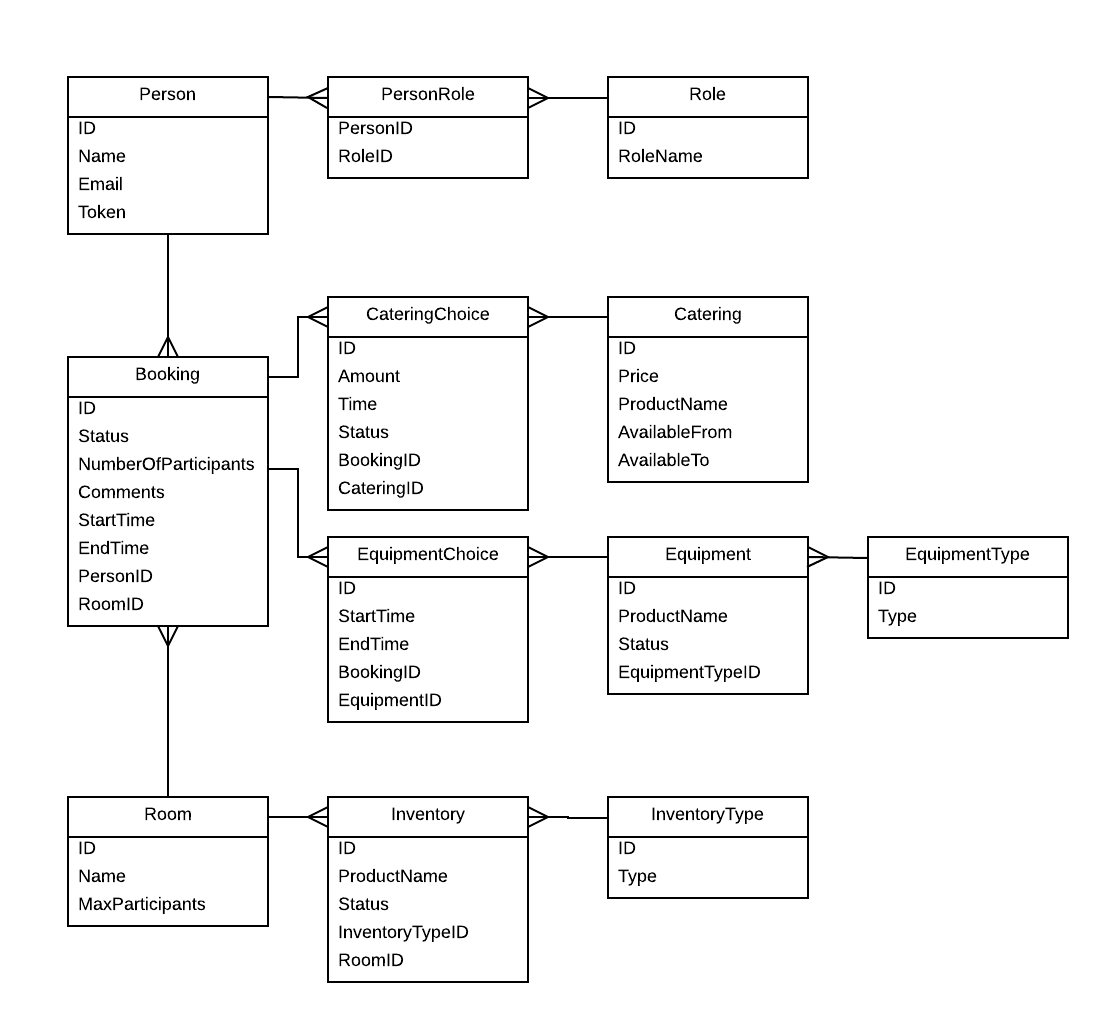
\includegraphics[width=\textwidth]{Chapters/Design/Technical/Images/OurDataModel}
  \caption{Datamodellen til vores løsning}
\label{Fig:Technical_Database_our_datamodel}
\end{figure}

\section{Servicen}
\label{Technical_Service}

\section{Klienten}
\label{Technical_Client}
\subsection*{Arkitektur}
\label{Technical_Client_Archi}
Vi har implementeret vores klient med en \textit{Model-View-ViewModel}\footnote{http://msdn.microsoft.com/en-us/magazine/dd419663.aspx} (\textit{MVVM}) arkitektur. Klassisk \textit{MVVM} bruger et \textit{ViewModel} lag til at separere modellen og brugergrænsefladen. \textit{ViewModel} laget skal fungere som oversætter for brugergrænsefladen og modellen, således at der ingen kontakt er mellem dem. 

I vores implementering har hvert \textit{View} en \textit{ViewModel}, som laver det meste af logikken (opdatering af gitrene, konstruktion af nye booking objekter, m.m.). \textit{View}s styrer selv, hvad der skal kaldes på dens tilhørende \textit{ViewModel} ved forskellige events.

Normalt er modellen i \textit{MVVM} en database, men da vi anvender det i forbindelse med en service, bruger vi service interfacet som model i stedet for vores database. Dette betyder i realiteten, at modellen bliver delt op i fire lag, hvis man ser den som en helhed (klient model, service interface, logik til databasekald og databasen selv). Hvis vi ikke havde lavet en service, ville man kunne have reduceret dette til et eller to lag, og dermed er mængden af nødvendig kode langt mindre.

Vi har desværre ikke opfyldt vores mål om at have en \textit{MVVM} arkitektur i den grad, som vi ønskede. Figur \ref{Fig:Technical_Client_Archi_nsd} illustrerer afhængigheder for vores namespaces i klienten. Hvis \textit{MVVM} arkitekturen skulle være opfyldt i helhed, ville hverken \textit{GUI} eller \textit{ViewModel} være afhængig af \textit{BookItService}.

\begin{figure}[h!]
  \centering
    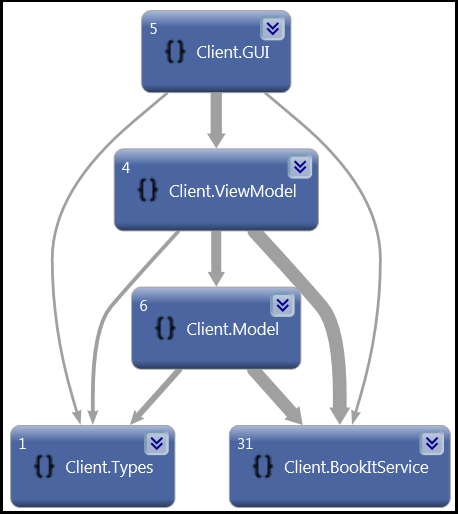
\includegraphics[width=0.4\textwidth]{Chapters/Design/Technical/Images/NamespaceDependencies}
  \caption{De forskellige lag i klienten og deres afhængigheder.}
\label{Fig:Technical_Client_Archi_nsd}
\end{figure}

\subsection*{Implementering af brugergrænsefladen}
\label{Technical_Client_GUI}
Klientens brugergrænseflade er udviklet i ASP.net\footnote{http://www.asp.net/} Web Forms og er kodet i C\#. Vi kalder vores brugergrænseflade for "klienten", selvom den er hostet serverside. Dette gør vi, fordi det er en "klient" til vores system. Vores klient skal stadig hostes af en server, som udfører det meste af klientens funktionalitet.

 Vores \textit{View}s består af .apsx filer, som beskriver udseendet af vores brugergrænseflade. Hvert \textit{View} har desuden en code-behind fil, som beskriver funktionaliteten af knapper og andre elementer på siden. Desuden har vi en \textit{Master Page}, som sørger for, at vi anvender et konsistent design.
\\Derudover anvender vi Cascading Style Sheets til at hjælpe med det konsistente design og Javascript til funktionalitet, som skal udføres af brugerens browser i stedet for serveren, som hoster klienten.

\section{Kodeeksempler}
\label{Technical_CodeExamples}
\chapter{Test af systemet}
\label{Test}
I dette kapitel beskriver vi vores test strategi og resultaterne af vores tests. Derudover diskuterer vi, hvad vi kunne have gjort anderledes og den strategi, vi gerne ville have indført, hvis vi havde haft mere tid.
\\En liste af de test, vi har udført findes i appendixafsnit \ref{App_Test_ListOfTest}. En liste af defekter i systemet findes i appendixafsnit \ref{App_Test_Defects}.

\section{Udført teststrategi}
\label{Test_strat}
Vi har udført en række test af vores brugergrænseflades funktionalitet. Disse test består af både postive og negative test af navigering og funktionalitet. Desuden tester vi, om det er muligt at udføre de arbejdsopgaver, vi understøtter (beskrevet i afsnit \ref{Evaluation_workareas}).

Vores test af navigering og funktionalitet er delt op per skærmbillede. Testene til hvert skærmbillede består hovedsageligt af test af knapper. De positive test skal undersøge, om brugergrænsefladen gør det, som den er beregnet til. Modsat skal de negative test undersøge, om brugergrænsefladen gør noget, som den ikke bør.

Vi skrev vores test efter vi havde implementeret brugergrænsefladen. Dette betød, at vi ikke forsøgte at rette fundne defekter. Vi har i stedet  tilføjet de fundne defekter til vores "future release"-liste.

\section{Resultater}
\label{Test_Results}
Vi har udført 78 test af vores system. 12 af disse er test i forbindelse med de arbejdsopgaver, vi understøtter (se afsnit \ref{Evaluation_workareas}). De resterende 66 test er test af vores skærmbilleder.

22 af vores test har status "OK", 35 rapporterer en defekt og 21 rapporterer "Not Yet Implemented". Dette betyder, at $\sim$28\% af vores er "OK". Dette er lav værdi, men den bliver over 50\% ($\sim$55\%), hvis man medregner de test, som rapporterer "Not Yet Implemented". 

Vi har valgt ikke at inkludere "Not Yet Implemented" i vores liste af defekter, da vi mener, der er forskel på test, som fejler på grund af bugs og test, der fejler grundet manglende implementation. 

\subsection{Vurdering af resultater}
\label{Test_Results_eval}
Det er skuffende for os, at vi har så få test, som har status "OK". Selvom det sjældent er muligt at konstruere et system, hvor alt funktionalitet er testet og alle test har status "OK", så er det stadig et mål for os i forbindelse med future releases. 
\\Vi vurderer, at det er muligt implementere det meste af den funktionalitet, hvis test fejler på grund af, at de ikke er implementeret. Dette ville bringe systemet tættere på 50\% godkendte test. 50\% godkendte test er dog stadig ikke nok til, at vi mener, at produktet ville være klar egentlig release. Derfor mener vi, at der bør lægges stor vægt på at få fixet størstedelen af de rapporterede defekter, før man fokuserer på tilføjelse af nye funktionaliteter.

Vi ville muligvis have været i stand til at reducere antallet af defekter, hvis vi havde skrevet vores test efter vi designede brugergrænsefladen, men før vi implementerede den. Testene beskriver mange af de forskellige input, som brugeren kan give til brugergrænsefladen. 
\\Risikoen ved dette er, at vores implementation ville blive så fokuseret på at opfylde testkravene, at vi ikke fik skrevet god kode. Eksempelvis kunne vi ende op med kode, som var fokuseret på at bestå individuelle test. Kode, som er fokuseret på enkelte cases, kan være svært at udvide og/eller vedligeholde.

\section{Ønsket teststrategi}
\label{Test_intendedStrat}
Hvis vi havde mere tid, ville vi have indført en mere grundig teststrategi. Denne test strategi består af flere typer af test samt en anden tilgang til testproceduren. Testene vil både være automatiske (test skrevet i kode) eller manuelle (en bruger sidder og udfører dem manuelt).

Testproceduren til vores ønskede teststrategi er fokuseret på at beskrive en række test til hver arbejdsopgave tidligt i processen. Mange af forretningsreglerne burde indgå som test eller dele af test. For eksempel bør det være en negativ test, at man ikke kan booke på samme tidspunkt, som en anden bruger har booket.
\\Derudover vil det være målet, at hver funktion har en række test (positive og negative), som skrives før selve funktionaliteten implementeres. I denne forbindelse er det vigtigt, at man får defineret, hvad funktionen skal gøre, da man ellers ville blive tvunget til at skrive testene om, hvis man laver ændringer i funktionaliteten.

Ydeligere vil vi anvende \textit{Code Contracts}\footnote{http://research.microsoft.com/en-us/projects/contracts/}. \textit{Code Contracts} gør det muligt at udtrykke krav til input, løfter om output samt objekt invarianter som en del af koden (i stedet for i dokumentationen). Der er to store fordele ved at anvende \textit{Code Contracts}. 

For det første gør \textit{Code Contracts} koden nemmere at implementere, da man har brug for langt færre if-statements til fx at undersøge korrekthed af input og output.
\\Derudover gør \textit{Code Contracts} det muligt at anvende "PEX and Moles"\footnote{http://research.microsoft.com/en-us/projects/pex/}. Pex finder interessante input/output værdier til metoder. Disse kan så gemmes som testsuites, hvilket gør det nemt at teste, om en metode gør det, den skal. Det er ikke nødvendigt at have \textit{Code Contracts} for at anvende PEX, men det gør det nemmere for PEX at generere meningsfulde test. PEX test kan dog ikke erstatte håndskrevne test, men de kan supplere kodedækningen af de håndskrevne test.

\subsection{Testtyper}
\label{Test_intendedStrat_types}
Vores ønskede strategi består af flere niveauer af tests:
\begin{my_description}
\item[Unit] Test af mindre dele af koden (fx enkelte metodekald).
\item[Scenario] Består af test, som kombinerer flere funktioner.
\item[Service] Test af forbindelse samt regler for input til servicekald.
\item[Brugergrænseflade] Test af navigering og arbejdsopgaver i brugergrænsefladen.
\end{my_description}

\subsubsection{Unit}
\label{Test_intendedStrat_types_unit}
Vores unit-test vil hovedsageligt bestå af den testsuite, som PEX genererer. Vi mener ikke, at det er nødvendigt at lave håndskrevne unit-test, medmindre de andre test i systemet ikke dækker alle kritiske dele af en funktion.

\subsubsection{Scenario}
\label{Test_intendedStrat_types_sce}
Scenario-test er test, som udfører en kombination af funktioner for at simulerere en kortere arbejdsopgave. Disse test er håndskrevne automatiske test, som ikke bliver udført gennem brugergrænsefladen. Kaldene vil typisk være til enten Service klassen\footnote{Testen ville blive udført direkte igennem projektet og ikke som kald til servicens webinterface.} eller entitets klasserne i vores service. Ydeligere kunne en scenario-test være test udført på model klasserne i klienten. 
\\Et eksempel på en scenario-test kunne være "Log ind og opret en booking".

\subsubsection{Service}
\label{Test_intendedStrat_types_service}
Vores service-test kalder servicens webinterface. Service-test fokuserer på tre elementer: forbindelse, problemer med data-bindings \& fejlhåndtering. De er ikke lige så fyldestgørende som scenario-test, da de kun tester de avancerede dele af hver service contract.

\subsubsection{Brugergrænseflade}
\label{Test_intendedStrat_types_UI}
Test af brugergrænsefladen kan både være automatiske og manuelle. De automatiske test vil bestå af simple test, hvor det forventede resultat altid er det samme (som fx navigering). De manuelle test vil bestå af de mere komplicerede opgaver, som udføres af brugeren.
\\"Log ind som testbruger og naviger til Dine Bookinger" kunne være en automatisk test af brugergrænsefladen.
\\"Log ind som testbruger, opret en booking, find bookingen i 'Dine Bookinger', slet bookingen" kunne være et manuel test af brugergrænsefladen.

\subsection{Regressionstest}
\label{Test_intendedStrat_regression}
Hvis vi (eller brugere af systemet) finder en fejl i systemet, er det planen at lave en test, som dækker præcis den case, som bliver beskrevet i forbindelse med fejlen. Det er meningen, at disse test skal fejle ved første kørsel for at sikre, at fejlen eksisterer samt, at testen er skrevet korrekt. Når fejlen er rettet, vil testen ikke længere fejle.
\\Da regressionstestene allerede er designet, beholder vi dem som en del af vores test. Dette sørger for, at fejlen ikke opstår på et senere tidspunkt i udviklingsprocessen.

\subsection{Kodedækning}
\label{Test_intendedStrat_coverage}
Det er sjældent en effektiv strategi at teste alt sin kode, da det er meget tidskrævende (både i design og udførelsen af testene). Vi mener, man bør teste indtil, man dækker en stor del af funktionaliteten uden, at det bliver redundant at teste yderligere. 
\\Vi vil anvende kodedækning\footnote{Der findes forskellige værktøjer til at måle kodedækning. Vi har tidligere anvendt DotCover (http://www.jetbrains.com/dotcover/).} til at sørge for, at vi tester vores system grundigt. Udover at vi skal have dækning af arbejdsopgaverne, så har vi følgende mål for kodedækning:
\begin{my_itemize}
\item \textbf{Service}
\item Mindst 50\% dækning af servicen.
\item Målet er 85\% dækning af servicen.
\item \textbf{Klient}\footnote{Det er sværere at måle kodedækning i klienten, da en stor del af klientens funktionalitet foregår i koden til brugergrænsefladen, som kan være svær at måle kodedækning for.}
\item Mindst 30\% dækning af klienten.
\item Målet er 65\% dækning af klienten. 
\end{my_itemize}

Disse mål burde sikre, at størstedelen af koden bliver testet. Hvis dækningen af service eller klient er lavere end vores mindstekrav, mener vi ikke, at systemet ikke tilstrækkeligt testet.
\chapter{Vurdering af vores løsning}
\label{Evaluation}

\section{Understøttelse af arbejdsopgaver}
\label{Evaluation_workareas}
Denne sektion beskriver hvilke arbejdsopgaver vi understøtter i første release samt giver en prioritering af, hvilke arbejdsopgaver der bør fokuseres på i følgende releases.

Kravspecifikationen definerer 13 arbejdsopgaver:
\begin{my_enumerate}
\item[\textbf{C01.}]{Administrer booking}
\item[\textbf{C02.}]{Forespørg på booking}
\item[\textbf{C03.}]{Modtag forespørgsel fra Ekstern}
\item[\textbf{C04.}]{Klargør lokaler}
\item[\textbf{C05.}]{Udlevér nøgle}
\item[\textbf{C06.}]{Håndtér forplejning}
\item[\textbf{C07.}]{Fakturér forplejning}
\item[\textbf{C08.}]{Opdatér menukort}
\item[\textbf{C09.}]{Opdater listen for ekstra udstyr}
\item[\textbf{C10.}]{Opdatér lokaler}
\item[\textbf{C11.}]{Administrér bruger}
\item[\textbf{C12.}]{Håndter statistik}
\item[\textbf{C13.}]{Behandl faktura}
\end{my_enumerate}

Ud af de 13 arbejdesopgaver understøtter vi \textbf{C01}, \textbf{C09} og \textbf{C10}.
\\Hver af arbejdsopgaverne har en række underpunkter, som beskriver delopgaver og varianter af disse delopgaver.

\textbf{C01:} Administrer booking\\
\textbf{Brugere:} Ansatte og studerende på ITU.\\
\textbf{Hyppighed:} Flere gange om dagen i alt for både studerende og ansatte.\\
\textbf{Start:} En person går ind i booking systemet for at booke, ændre eller få overblik over bookinger.\\
\textbf{Slut:} Når bookingen eller lændringen er foretaget.

\begin{tabular}{ | l | l | l | l | p{5} |}
\hline
	Arbejdesopgave & Understøttet & Eksempel løsning & Vores løsning\\ 
\hline
	C1.1 Søg efter ledigt tidspunkt for ny booking & Ja & & Skærmbillede \ref{Design_G_Development_FinalGrid} på side \pageref{Design_G_Development_FinalGrid} \\ 
\hline
	C1.1a Søg efter eksisterende booking & Ja & &Skærmbillede \ref{Design_G_Development_YourBookings_Final} på side \pageref{Design_G_Development_YourBookings_Final}\\ 
\hline
	C.2 Vælg ledigt lokale, forplejning og ekstra udstyr & Ja & &Skærmbillede \ref{Design_G_Development_Forplejning_Final} på side \pageref{Design_G_Development_Forplejning_Final}\\ 
\hline
	C1.2a Vis eksisterende booking(er) & Ja & &Skærmbillede \ref{Design_G_Development_FinalGrid} på side \pageref{Design_G_Development_FinalGrid}\\ 
\hline
	C1.3 Opdater booking & Ja & &Skærmbillede \ref{Design_G_Development_FinalGrid} på side \pageref{Design_G_Development_FinalGrid}\\ 
\hline
	C1.4 Annuller booking & Ja & &Skærmbillede \ref{Design_G_Development_YourBookings_Final} på side \pageref{Design_G_Development_YourBookings_Final}\\ 
\hline
	C1.5 Opret booking & Ja & &Skærmbillede \ref{Design_G_Development_FinalGrid} på side \pageref{Design_G_Development_FinalGrid}\\ 
\hline
\end{tabular}

\textbf{C09:} Opdater listen for ekstra udstyr\\
\textbf{Brugere:} Facility Management (FM)\\
\textbf{Hyppighed:} Når der sker ændring i udvalget af ekstra udstyr (en gang om måneden)\\
\textbf{Start:} Når der er behov for at udstyrslisten skal opdateres\\
\textbf{Slut:} Når listen er opdateret

\begin{tabular}{ | l | l | l | l | p{5} |}
\hline
	Arbejdesopgave & Understøttet & Eksempel løsning & Vores løsning\\ 
\hline
	C9.1 Rediger udstyrslisten & Ja & FM er ansvarlig & Skærmbillede \ref{Design_G_Development_UdstyrsListe_Final} på side \pageref{Design_G_Development_UdstyrsListe_Final} \\ 
\hline
\end{tabular}

\textbf{C10:} Opdatér lokaler\\
\textbf{Brugere:} Facility Management (FM)\\
\textbf{Hyppighed:} Når der sker ændring i antallet af lokaler til bookingen (en gang om måneden)\\
\textbf{Start:} Når der er behov for at lokalelisten skal opdateres\\
\textbf{Slut:} Når listen er opdateret

\begin{tabular}{ | l | l | l | l | p{5} |}
\hline
	Arbejdesopgave & Understøttet & Eksempel løsning & Vores løsning\\ 
\hline
% Der skal være ref til superlokaleliste som kommer til at ligge i appendix
	C10.1 Rediger lokalelisten & Ja & & Skærmbillede \ref{} på side \pageref{} \\ 
\hline
	C10.2 Rediger lokale inventar & Ja & & Skærmbillede \ref{Design_G_Development_AendreLokale_Final} på side \pageref{Design_G_Development_AendreLokale_Final} \\ 
\hline
\end{tabular}

\subsection{Prioritering af arbejdsopgaver}
\label{Evaluation_workareas_priorities}
Vi valgte til den første release af systemet at priotere

Til den første release af systemet valgte vi at fokusere på at understøtte systemadministration og booking af lokaler og udstyr, hvilket tydeligt kan ses i afsnit \ref{Baggrund_Arb_opgaver} da alle arbejdsopgaverne i arbejdsområderne \textbf{C1},\textbf{C9} og \textbf{C10} er understøttet. 

I kravspecifikationen er de arbejdsområder også blandt dem som er vægtet højest og det er samtidig de arbejdsområder som indeholder kernefunktionerne i systemet. Det som ikke blev prioriteret højt nok til at komme med i første release var de arbejdsopgaver som fokuserede på integrationen med kantinen, samt mulighed for fakturing og statestik , arbejdsopgaverne \textbf{C6}, \textbf{C7}, \textbf{C12} og \textbf{C13} er eksempler på sådanne opgaver.
\\Grunden til, at vi ikke tog de arbejdsopgaver med var, at vi vurderede, at de ikke var nødvendige for at have et system der understøttede basis funktioner, derudover lagde arbejdsopgaverne op til, at der skulle implementeres et interface specifikt til kantinen hvilket vi vurderede ville tage lang tid at implementere og vi ville også have tre brugergrupper at tage hensyn til ift. usability og testing.

Fokus for næste release vil derfor være at få udarbejdet et interface som kantinen kan bruge til at integrere med resten af systemet og få finpudset de allerede eksisterende funktioner i kravspecifikationen. Behandling af faktura har også en høj vægtning, så det vil der også blive lagt fokus på. 
\chapter{Alternative Systemer}
\label{Comparison}
Udover at udvikle vores udgave af et booking-system til IT-Universitetet, vil vi i dette kapitel give en kort beskrivelse af to alternative  systemer og sammenligne dem med vores løsning.

\section{Room Booking System}
\label{Comparison_RBS}
"Room Booking System"\footnote{http://www.roombookingsystem.co.uk/} er et web-baseret booking system designet til at opfylde både skoler og virksomheders behov. 

Interfacet er designet som en kalender, hvor man kan vælge hvilke kategorier af ressourcer man kan vil se tider for eksempelvis, IT rum, mødelokaler, projekter eller andet udstyr. Bookinger af diverse ressourcer er ligesom vores system opgjort i farvekoder så man hurtigt kan få et overblik over hvad der er ledigt og hvad der er booket. Figur \ref{Comparison_RBS_RoomBookingSystem} visser det først skærmbillede i "Room Booking System"

\begin{figure}[h!]
  \centering
    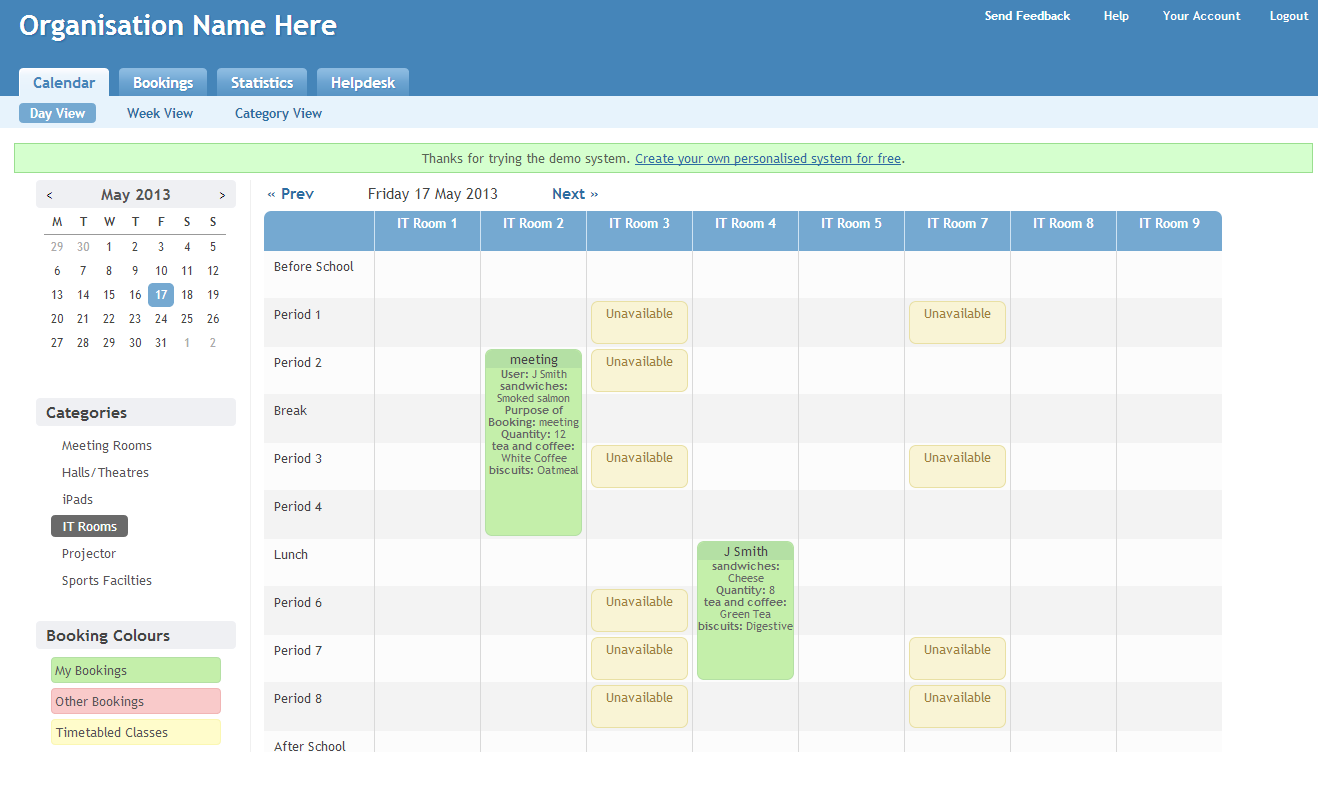
\includegraphics[width=0.8\textwidth]{Appendix/GUI-Prototype/RoomBookingSystem}
  \caption{Det først skærmbillede i systemet som visser oversigten over booket ressourcer}
\label{Comparison_RBS_RoomBookingSystem}
\end{figure}

"Room Booking System" giver også mulighed for tilføje forplejning til ens bookinger. Figur \ref{Comparison_RBS_RoomBookingSystemList} visser skærmbilledet der svare til vores booking-liste, her kan det ses at der til bookingen er blevet bestilt sandwicher med røget laks plus te og kiks.

\begin{figure}[h!]
  \centering
    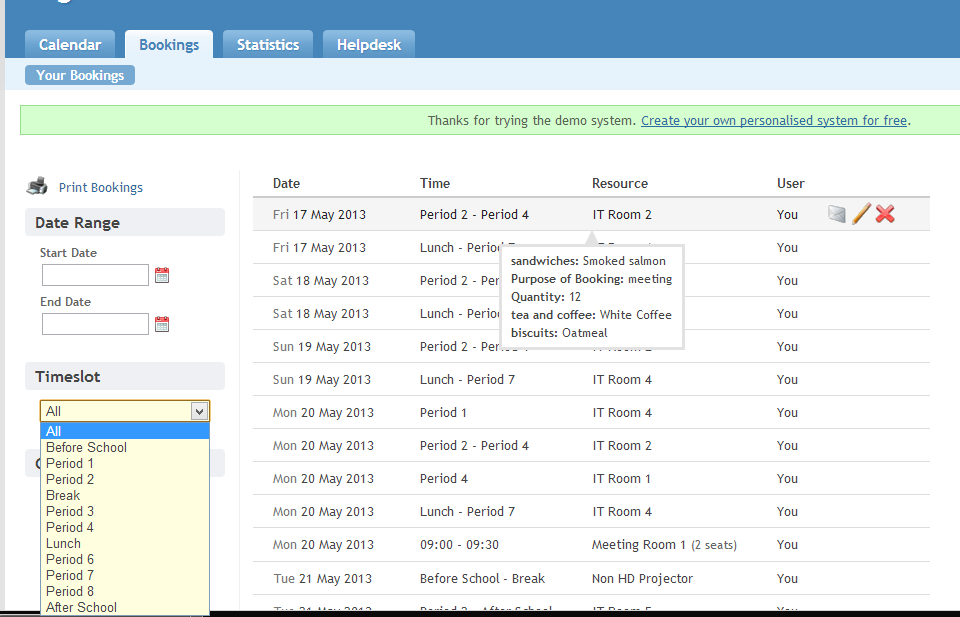
\includegraphics[width=0.8\textwidth]{Appendix/GUI-Prototype/RoomBookingSystemList}
  \caption{Skærmbillede over de bookinger der i systemet}
\label{Comparison_RBS_RoomBookingSystemList}
\end{figure}

Desuden er login til systemet seperat og dermed er der ikke mulighed for at integrere det med hverken Active Directory (AD) eller Where Are You From (WAYF). Et abonnement, der understøtter 200 lokaler/udstyr og 500 brugere, koster 434 kr. om måneden.

En fordel ved "Room Booking System" er, at det giver mulighed for at lave statistikker se figur \ref{Comparison_RBS_RoomBookingSystemStatistic}. Desuden kan det ses som en fordel, at det er hostet eksternt.

\begin{figure}[h!]
  \centering
    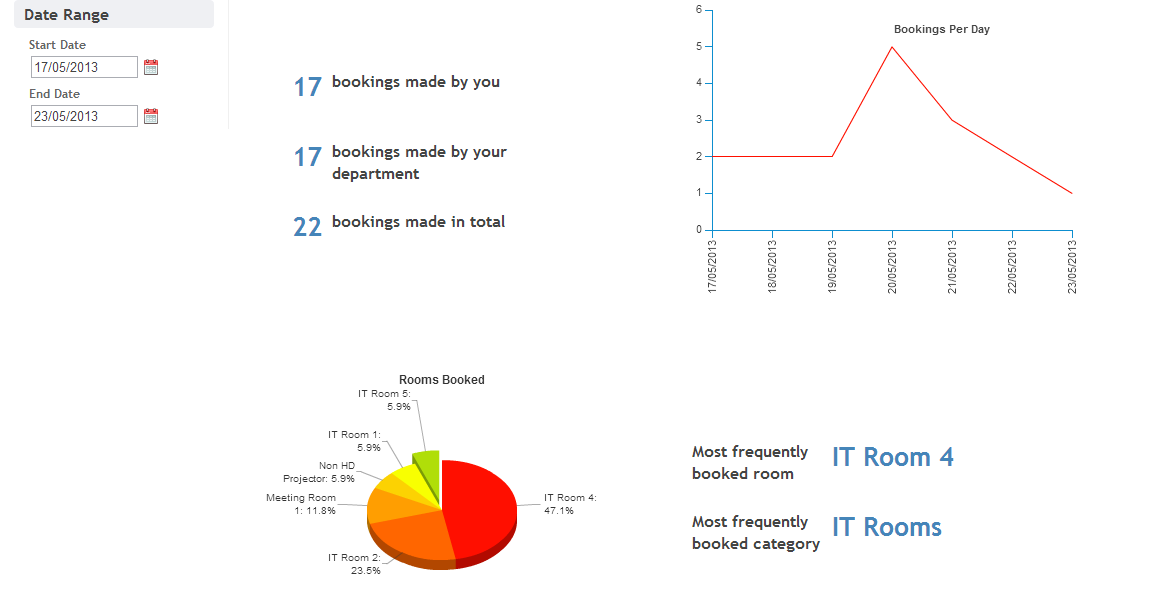
\includegraphics[width=0.8\textwidth]{Appendix/GUI-Prototype/RoomBookingSystemStatistic}
  \caption{Skærmbillede til visning af statestik over booking af ressourcer.}
\label{Comparison_RBS_RoomBookingSystemStatistic}
\end{figure}

Ulempen ved "Room Booking System" i forhold til vores løsning er, at der er en grænse for hvor mange lokaler og udstyrselementer, som kan bookes i systemet. Desuden er det ikke muligt at integrere med et eksisterende ITU login system. Da der kun er mulighed for 500 brugere i systemet, vil nogle brugere skulle slettes for, at der kan oprettes nye i forbindelse med nye studerende/ansatte.

Hvis man vil afprøve systemet er der i menubaren på hjemmesiden et punkt der hedder demo. Der kan man frit prøve og undersøge interfacet og dets feature uden at skulle oprette bruger eller downloade nogen klient.

\section{School Booking}
\label{Comparison_SB}
"School Booking"\footnote{http://www.schoolbooking.com/} er et andet web-baseret system, som primært er designet til brug af skoler. 

Systemet giver mulighed for at booke både lokaler og udstyr\footnote{Det bookede udstyr kan være forplejning, hvis man sætter rigtigt op.}. Man kan betale ekstra for at tillade eksterne bookere. Statetisk er også muligt i dette system. Der er dog ikke mulighed for at integrere det med AD eller WAYF.

Et system, der understøtter 1000 brugere, 300 lokaler/resurser, eksterne bookere og statestik koster årligt ~11.500 kr.

Fordelen ved dette system er det samme som ved "Room Booking System": muligheden for at lave statestik.

Ulempen ved dette system er, at der er en begrænset mængde af brugere, som kan anvende systemet, samt at det ikke er muligt at integrere det med AD eller lignende, fordi det er hostet eksternt.

Vi har desvære ingen mulighed for at undersøge brugervenligheden af systemet da der ikke var nogen offentlige screenshots og det krævede at man skulle være en registrer bruger for, at man kunne prøve deres 30 dags gratis prøveperiode.
\chapter{Lessons learned}
\label{Conclusion_Lessons}
\section{Kravspecifikationen}
\label{Lessons_Krav}
I begyndelsen af projektet så vi kravspecifikationen som en række af fejlfri krav, som ikke kunne diskuteres eller bøjes. Vi forsøgte at følge kravspecifikationen i dets fulde omfang i stedet for at opfylde de krav, som vi mente var de vigtigste.

Da vi havde nærlæst kravspecifikationen, fandt vi ud af, at der var nogle problemer i den. For eksempel har vi lavet nogle rettelser i datamodellen, som var nødvendige i forbindelse med at lave en god implementering af systemet.

Lektien for os har været, at udvikleren skal være opmærksom på, hvad kravspecifikationen indeholder, og være klar til at diskutere kravene med kunden, så man er sikker på, at det bedste produkt bliver lavet. Desuden bør man diskutere en prioriteringsliste med kunden, således at kunden er sikker på, at udvikleren laver det vigtigste først.

\section{Projekter af samme natur er ikke nødvendigvis ens}
\label{Lessons_Projekt}
Da vi begge havde været med til at udvikle et system til filmudlejning, endte vi med at undervurdere, hvor meget arbejde der lå i implementeringen af vores design af bookingsystemet.

Systemet var udviklet i C\# med en WCF-service hooket op til en Microsoft SQL-database med en tilhørende klient. Da dette system delte mange af de samme elementer som systemet, vi har udviklet i forbindelse med dette projekt, vurderede vi, at det ikke ville være en særligt stor omkostning at overføre meget af funktionaliteten til vores bookingsystem.

Vi glemte at tage med i vores vurdering, at vi var fem personer på det forrige projekt, og derfor havde vi specialiseret os i forskellige dele af systemet. Da vi kun var to personer til dette projekt, betød det, at vi manglede erfaringen fra de personer fra det forrige projekt, som havde specialiseret sig inden for de ting, som vi ikke havde haft fokus på. Dette betød, at vi selv blev nødt til at tilegne os viden fra de felter, som de havde stået for. Dette gjorde, at vores vurdering af omkostningerne for vores valgte løsning var forkert.

Lektien i denne forbindelse har været, at man skal passe på med at fejlvurdere, hvor meget erfaring fra tidligere projekter kan gavne en i et andet projekt, selvom projekterne er meget ens.

\section{En service er ikke altid den rigtige løsning}
\label{Lessons_Service}
I forbindelse med vores valg af implementeringsstrategi, lavede vi en vurdering af, hvor meget det ville gavne kunden (ITU), hvis vi udviklede en service som en del af systemet. Vi vurderede, at det ville være en stor fordel for kunden, hvis det var nemt at udvide systemet til flere platforme.

Den første udgave, som vi udviklede i forbindelse med dette projekt, havde dog slet ikke brug for en service. Vi burde i stedet have koblet vores klient direkte til databasen. 
\\Arkitekturen, vi anvender i klienten, gør det relativt smertefrit at koble klienten op til en service i stedet for direkte til databasen, hvis systemet senere skulle udvides.

Vi tog ikke med i vores overvejelser, at projektperioden var begrænset, så vi vurderede kun omkostningerne i vores cost/benefit-analyse i forhold til hinanden. Dette betød, at vi ikke havde lavet en egentlig vurdering af, om det var muligt for os at nå at udvikle både service og klient.

I fremtidige projekter vil vi sørge for at vurdere, om der overhovedet er brug for avancerede features (fx en service) i forhold til kundes behov.

\section{Projektstyring}
\label{Lessons_Styring}
Vores styring af projektet har været meget løs og parallel. 

Det havde været en fordel for vores projekt, hvis vi havde haft delmilestones eller en iterativ styringsmodel. Vi ville have haft bedre styr på, hvor meget vi manglede på et givent tidspunkt i processen. Desuden ville vi haft mere materiale at få feedback på fra vores vejleder.

Da vi har arbejdet meget parallelt, har vi ikke været gode nok til at holde hinanden opdateret på, hvor man var i forbindelse med det, man arbejdede på. Når vi endelig tog beslutninger, blev de ikke dokumenteret ordenligt.

Vi manglede et fælles beslutningspapir, som var til rådighed for os begge, hvor vi skrev alle vores beslutninger ned i forhold til tekniske og grafiske designbeslutninger. Dette ville også have hjulpet os i forhold til vores meget parallelle arbejdsgang, da man ville have mulighed for at konsultere beslutningspapiret i stedet for at forstyrre den, man arbejder sammen med.

Lektien, vi har lært i denne forbindelse, har været, at selvom man arbejder parallelt, er det stadig vigtigt at have fælles mål. Derudover er det vigtigt at sørge for, at der stadig bliver kommunikeret mellem gruppemedlemmerne og sørge for, at den kommunikation bliver dokumenteret, så man kan støtte sig op af den senere i processen.
\begin{thebibliography}{9}
\bibitem[SL]{SL_UID} Lauesen, Søren. User Interface Design, A Software Engineering Perspective. Great Britain: Pearson Educated Limited, 2005.  Print.
\bibitem[KravSpec]{kravspec} Miki Ipsen, Garwun Jeffrey Lai, Merete Larsen, Stig Larsen. Kravspecifikation til ITU Booking System. December, 2012.
\end{thebibliography}
\label{A_BIB}
\appendix
\addappheadtotoc
\appendixpage
\settocdepth{chapter}
\label{App}
\chapter{System Diagrammer}
\label{App_Diagrams}
\chapter{Skærmbilleder}
\label{App_GUI}

\section{Paper mockup}
\label{App_GUI_paper}

\section{Endelige skærmbilleder}
\label{App_GUI_final}
\chapter{Udvalgte Dele Af Koden}
\label{App_Code}
\section{SQL-kode til oprettelse af database}
\label{App_Code_DBC}
\section{BookItModel.cs}
\label{App_Code_BookingModel}
\section{RoomListViewModel.cs}
\label{App_Code_RoomList}
\section{Booking.cs}
\label{App_Code_BookingEntity}
\section{BookItContext.cs}
\label{App_Code_Context}
\section{BookItContext.cs}
\label{App_Code_Context}
\section{Configuration.cs}
\label{App_Code_Conf}

%\chapter{Test resultater}
\label{Test results}

\end{document}